% Appendix of main.tex (\input after the bibliography). Main text: main.tex. One writer: the appendix owner.
% v6 order follows the reader's questions: A proofs, B reach emulation, C implementation and pseudocode,
% D evaluation protocol and baselines, E extended results (Tables 1 and 2 expanded), F progressive SCA,
% G generality (Table 3 expanded), H sensitivity and budgets, I compute and reproducibility, J limitations,
% K prompts, L sample pages. Every label of v5.1 is kept; v6 adds subsection labels (listed in
% .agent/notes/paper_v6/appendix.md).
% =====================================================================================
\clearpage
\appendix
\raggedbottom
\topfloatpages
\counterwithin{figure}{section}
\counterwithin{table}{section}
% Float placement for the appendix only (the main text has been flushed by the \clearpage above).
\setcounter{topnumber}{3}\setcounter{bottomnumber}{2}\setcounter{totalnumber}{5}
\renewcommand{\topfraction}{0.95}\renewcommand{\bottomfraction}{0.7}
\renewcommand{\textfraction}{0.05}\renewcommand{\floatpagefraction}{0.6}

% ---- Helpers ---------------------------------------------------------------------------
% Text that names a progressive gallery appears only once its snippet exists (visuals owner).
\newcommand{\ifprogGallery}[1]{\IfFileExists{figures/snippets/gallery_prog.tex}{#1}{}}
\newcommand{\ifprogSixteen}[1]{\IfFileExists{figures/snippets/gallery_prog16.tex}{#1}{}}
% A figure file: the v6 version under figures/v6/ when it exists, else the v5.1 file, else a visible placeholder.
\newcommand{\apxgraphic}[2][width=\linewidth]{%
  \IfFileExists{figures/v6/#2.pdf}{\includegraphics[#1]{figures/v6/#2.pdf}}{%
  \IfFileExists{figures/#2.pdf}{\includegraphics[#1]{figures/#2.pdf}}{%
  \fbox{\parbox{0.9\linewidth}{\centering\footnotesize\texttt{\detokenize{#2}} pending}}}}}
% A generated table body (figures/snippets/<stem>.tex), or a visible placeholder while it does not exist.
\newcommand{\apxbody}[1]{\snippet{#1}{\centering\fbox{\parbox{0.9\linewidth}{\centering\footnotesize\texttt{\detokenize{#1}} pending}}}}
% \apxinput{placement}{file}: input a float snippet file with its float placement replaced.
% \snippetat{placement}{stem}: the snippet figures/snippets/<stem>.tex, nothing if it is absent.
% \vsnippet{placement}{stem}: the v6 snippet figures/v6/snippets/<stem>.tex when it exists, else \snippetat.
\makeatletter
\newcommand{\apxinput}[2]{\begingroup\def\sca@place{#1}%
  \let\sca@fig\figure\let\sca@tab\table\expandafter\let\expandafter\sca@figs\csname figure*\endcsname
  \renewcommand{\figure}[1][]{\expandafter\sca@fig\expandafter[\sca@place]}%
  \renewcommand{\table}[1][]{\expandafter\sca@tab\expandafter[\sca@place]}%
  \expandafter\renewcommand\csname figure*\endcsname[1][]{\expandafter\sca@figs\expandafter[\sca@place]}%
  \let\apx@origlabel\label
  \def\label##1{\apx@origlabel{##1}\@ifundefined{apx@alias@##1}{}{%
    \edef\apx@tmp{\csname apx@alias@##1\endcsname}\expandafter\apx@origlabel\expandafter{\apx@tmp}}}%
  \input{#2}\endgroup}
\newcommand{\snippetat}[2]{\IfFileExists{figures/snippets/#2.tex}{\apxinput{#1}{figures/snippets/#2.tex}}{}}
\newcommand{\vsnippet}[2]{\IfFileExists{figures/v6/snippets/#2.tex}{\apxinput{#1}{figures/v6/snippets/#2.tex}}{\snippetat{#1}{#2}}}
% \apxalias{label}{alias}: a snippet float that sets <label> also sets <alias> (a retired label kept alive).
\newcommand{\apxalias}[2]{\global\@namedef{apx@alias@#1}{#2}}
% Captions of the v6 sample figures: the snippet (visuals owner) keeps its selection and crop clauses; the appendix
% owns the claim. \apxcap{n}{lead}{close} replaces the bold lead of the n-th caption of the next \vsnippetcap and adds
% the sentence <close> at its end (empty: none). The v5.1 fallback snippets keep their own captions.
\newcount\apx@capno
\newcommand{\apxcap}[3]{\global\@namedef{apx@lead#1}{#2}\global\@namedef{apx@close#1}{#3}}
\newcommand{\apx@clearcaps}{\@for\apx@n:=1,2,3\do{\global\expandafter\let\csname apx@lead\apx@n\endcsname\relax
  \global\expandafter\let\csname apx@close\apx@n\endcsname\relax}}
\def\apx@relead#1#2#3\apx@nil{#1{\csname apx@lead\the\apx@capno\endcsname}#3%
  \expandafter\ifx\csname apx@close\the\apx@capno\endcsname\@empty\else\space\csname apx@close\the\apx@capno\endcsname\fi}
% The text format apxlead, defined directly (\DeclareCaptionTextFormat is preamble-only; caption3 stores a text
% format as \caption@textformat@<name>).
\long\expandafter\gdef\csname caption@textformat@apxlead\endcsname#1{\expandafter\ifx\csname apx@lead\the\apx@capno\endcsname\relax#1\else\apx@relead#1\apx@nil\fi}
\newcommand{\vsnippetcap}[2]{\IfFileExists{figures/v6/snippets/#2.tex}{\begingroup\global\apx@capno\z@
    \let\apx@origcaption\caption\def\caption{\global\advance\apx@capno\@ne\apx@origcaption}%
    \captionsetup{textformat=apxlead}\apxinput{#1}{figures/v6/snippets/#2.tex}\endgroup}{\snippetat{#1}{#2}}%
  \apx@clearcaps}
% \apxbarrier: the float barrier at every section. When the floats still waiting would fill more than
% about a page, it flushes them like \FloatBarrier. Otherwise it lets them appear at the top of the next
% page, so a section never ends on a page of a few stranded lines and no float drifts more than a page.
\newdimen\apx@pend
\newcommand{\apxbarrier}{\par\begingroup\global\apx@pend\z@
  \def\@elt##1{\global\advance\apx@pend\ht##1\global\advance\apx@pend\dp##1\global\advance\apx@pend\floatsep}%
  \@deferlist\endgroup
  \ifdim\apx@pend>0.9\textheight\relax\FloatBarrier\fi}
\makeatother
% \ifvsnip{stem}{text}{fallback}: text that describes the v6 version of a figure of the visuals owner, while
% the v5.1 figure (and the fallback text) is used until figures/v6/snippets/<stem>.tex exists.
\newcommand{\ifvsnip}[3]{\IfFileExists{figures/v6/snippets/#1.tex}{#2}{#3}}
% \iflabel{label}{text if the label exists}{text otherwise}: for main-text labels that the text owner may add or drop.
\newcommand{\iflabel}[3]{\ifcsname r@#1\endcsname#2\else#3\fi}
% \apxband{name}: a grey band row that names a group of settings (configuration tables).
\newcommand{\apxband}[1]{\rowcolor[HTML]{EEF0F2}\multicolumn{2}{@{}l}{\textbf{#1}}\\}
% \apxfloat{stem}{label}: a generated float snippet (figures/snippets/<stem>.tex) at [!htbp], or, while it is
% absent, a labelled placeholder table so that every reference still resolves.
\newcommand{\apxfloat}[2]{\IfFileExists{figures/snippets/#1.tex}{\snippetat{!htbp}{#1}}{%
  \begin{table}[!htbp]\caption{\texttt{\detokenize{#1}} pending.}\label{#2}\centering\fbox{\parbox{0.9\linewidth}{\centering\footnotesize\texttt{\detokenize{#1}} pending}}\end{table}}}
% Our rows and the reference column of a table: the pale method green of every table.
\newcommand{\apxshade}{\rowcolor[HTML]{EAF4F1}}
% Y{w}: centred cell of width w that sets a {\tiny[lo, hi]} interval on its own line below the estimate.
% Tables with inline intervals set \let\tiny\scriptsize for the same size. Used by panel46_deltas.tex too.
\newcolumntype{Y}[1]{>{\centering\arraybackslash\renewcommand\tiny{\endgraf\setlength{\baselineskip}{7pt}}}p{#1}<{\rule[-3pt]{0pt}{0pt}}}

% ---- Contents ----------------------------------------------------------------------------
% \apxS{label}{title}: a section line; \apxs{label}{title}: a subsection line. Page numbers follow the labels.
\newcommand{\apxS}[2]{\textbf{\ref{#1}}&\textbf{#2}\nobreak\dotfill\nobreak\textbf{\pageref{#1}}\\}
\newcommand{\apxs}[2]{&\makebox[1.9em][l]{\ref{#1}}#2\nobreak\dotfill\nobreak\pageref{#1}\\}
\newcommand{\apxgap}{\noalign{\vskip3pt}}
\newcommand{\newmodelsline}{}
\ifanynewmodel\renewcommand{\newmodelsline}{\apxs{app:newer}{Newer models}}\fi
\newcommand{\holmline}{}
\IfFileExists{figures/snippets/app_tables/holm.tex}{\renewcommand{\holmline}{\apxs{app:holm}{Multiple comparisons}}}{}

\section*{Appendix}
\noindent Each section opens with the part of the main text it expands. Floats are numbered by section: Table~E.2 is the second table of Appendix~E.

\vspace{4pt}
{\small\setlength{\tabcolsep}{2pt}\renewcommand{\arraystretch}{1.02}
\noindent\begin{minipage}[t]{0.485\linewidth}
\begin{tabular}[t]{@{}l>{\raggedright\arraybackslash}p{0.91\linewidth}@{}}
\apxS{app:proofs}{Proofs}
\apxgap
\apxS{app:emulation}{Reach emulation}
\apxs{app:emu_record}{What one pass records}
\apxs{app:emu_head}{The head sets the reach}
\apxs{app:emu_table}{The reach table}
\apxs{app:emu_error}{Output error of each rule}
\apxgap
\apxS{app:impl}{Implementation and pseudocode}
\apxs{app:zoom}{The operators in detail}
\apxs{app:code}{Pseudocode}
\apxs{app:kernel}{Kernel and numerics}
\apxs{app:cost}{Attention cost}
\apxs{app:hparams}{Hyperparameters}
\apxgap
\apxS{app:metrics}{Evaluation protocol and baselines}
\apxs{app:protocol}{Protocol and prompts}
\apxs{app:metricdefs}{Metrics}
\apxs{app:intervals}{Intervals and table conventions}
\apxs{app:timing}{Timing}
\apxs{app:samples}{Sample figures}
\apxs{app:related}{How each method changes attention}
\apxs{app:area}{AReA}
\apxs{app:additional_protocols}{Other baselines and FLUX.2-dev}
\end{tabular}
\end{minipage}\hfill
\begin{minipage}[t]{0.485\linewidth}
\begin{tabular}[t]{@{}l>{\raggedright\arraybackslash}p{0.91\linewidth}@{}}
\apxS{app:tables}{Extended results}
\apxs{app:allmetrics}{Every metric of Table~\ref{tab:main}}
\apxs{app:pairs}{Headline comparisons}
\holmline
\apxs{app:phase2}{Every baseline against \sca{}}
\apxs{app:abl}{Ablations}
\apxs{app:latency}{Latency}
\apxgap
\apxS{app:prog}{Progressive \sca{}}
\apxs{app:prog_protocol}{Protocol}
\apxs{app:prog_results}{Against HRDiT and single pass}
\apxgap
\apxS{app:generality}{Generality}
\apxs{app:gen_seeds}{Seeds, HRGen-1K, FLUX.2-dev}
\apxs{app:gen_krea}{$6144^2$ and FLUX.1-Krea-dev}
\apxs{app:wide}{Non-square sizes}
\apxs{app:8k}{Exploratory $8192^2$}
\newmodelsline
\apxgap
\apxS{app:budget}{Sensitivity and budgets}
\apxs{app:sens}{Emulation budget and gate}
\apxs{app:ps2}{Reach table at non-square sizes}
\apxs{app:budgets}{Steps, guidance, and SigMa}
\apxgap
\apxS{app:compute}{Compute and reproducibility}
\apxs{app:hardware}{Hardware and compute}
\apxs{app:release}{Release and sources}
\apxgap
\apxS{app:limits}{Limitations in detail}
\apxs{app:failures}{Failure cases and scope}
\apxs{app:impact}{Broader impact}
\apxgap
\apxS{app:prompts}{Emulation prompts}
\apxgap
\apxS{app:galleries}{Sample pages}
\end{tabular}
\end{minipage}}

% =====================================================================================
\apxbarrier
\section{Proofs}
\label{app:proofs}

This appendix proves the statements that Sections~\ref{sec:observation} and~\ref{sec:method} use. Lemma~\ref{lem:split} is the split behind the definition of reach. Propositions~\ref{prop:range} and~\ref{prop:cost} give the trained position range and the cost of the two views (Section~\ref{sec:branches}). The proof of Proposition~\ref{prop:opt} gives the closed-form fit and the price of any coarser rule (Section~\ref{sec:emulation}). Remark~\ref{rem:text} treats text-image offsets.

\begin{lemma}[Softmax split]
\label{lem:split}
Let the keys of a query be partitioned into a near set $\Kset^{\mathrm{near}}$ and a far set $\Kset^{\mathrm{far}}$, with logits $\ell_j$. Then $\Ofull=m\,O^{\mathrm{near}}+(1-m)\,O^{\mathrm{far}}$ with $m=\sum_{j\in\Kset^{\mathrm{near}}}e^{\ell_j}/\sum_{j}e^{\ell_j}$ and $O^{\mathrm{near}},O^{\mathrm{far}}$ the softmax outputs restricted to $\Kset^{\mathrm{near}}$ and $\Kset^{\mathrm{far}}$.
\end{lemma}
\begin{proof}
Write $Z^{\mathrm{near}}=\sum_{j\in\Kset^{\mathrm{near}}}e^{\ell_j}$, so that $Z^{\mathrm{near}}O^{\mathrm{near}}=\sum_{j\in\Kset^{\mathrm{near}}}e^{\ell_j}v_j$, and likewise for the far set. Then $\Ofull=(Z^{\mathrm{near}}O^{\mathrm{near}}+Z^{\mathrm{far}}O^{\mathrm{far}})/(Z^{\mathrm{near}}+Z^{\mathrm{far}})$, and $Z^{\mathrm{near}}/(Z^{\mathrm{near}}+Z^{\mathrm{far}})=m$.
\end{proof}
The lemma motivates the two-branch form; \sca{}'s key sets are not a partition. Block centres can fall inside the window, and text keys enter both branches. A bridge token inside the window appears twice in the local softmax, which doubles its weight there.

\begin{proposition}[Trained position range]
\label{prop:range}
Assume exact integer positions and $t\le n_0\le\min(H,W)$. Every query-key offset of the global operator, and every offset between an image query and a key of its native window $\Win_{n_0}(i)$ (bridge keys and wider windows excluded), is at most $n_0-1$ per axis. Each global-operator query sees the native $T+n_0^2$ keys.
\end{proposition}
\begin{proof}[Proof of Proposition~\ref{prop:range}]
\emph{Global operator.} Image queries sit at $c(p_i)\in\Gnat=[n_0]^2$ and text queries at $0\in\Gnat$; subsampled keys sit at $b\in\Gnat$ and text keys at $0$. Any two points of $[n_0]^2$ differ by at most $n_0-1$ per axis. The key count is $T+|\Gnat|=T+n_0^2$.

\emph{Local operator.} Fix one axis of length $H\ge w$ and a tile $[t\tau,\,t\tau+t)$ with $t\le w$. The unclamped start $a'=t\tau+\lfloor t/2\rfloor-\lfloor w/2\rfloor$ satisfies $a'\le t\tau$ because $\lfloor t/2\rfloor\le\lfloor w/2\rfloor$, and $a'+w\ge t\tau+t$ because $w-\lfloor w/2\rfloor=\lceil w/2\rceil\ge\lceil t/2\rceil=t-\lfloor t/2\rfloor$. If $a'<0$ the window is $[0,w)$, and $w\ge a'+w\ge t\tau+t$. If $a'>H-w$ the window is $[H-w,H)$, with $H-w<a'\le t\tau$ and $H\ge t\tau+t$. In every case the window contains the tile, so it contains each query of the tile, and two positions in a window of side $w\le n_0$ differ by at most $n_0-1$. The proposition makes no claim about the bridge keys, which keep their true positions.
\end{proof}

\begin{remark}[Text-image offsets]
\label{rem:text}
FLUX.1 places all text tokens at position 0, so the offset between an image query at $p_i$ and a text key is $p_i$. In the global operator the query sits at $c(p_i)\in[n_0]^2$, inside the trained range. In the local operator it keeps $p_i$, up to $sn_0-1$ per axis, exactly as in full attention and in AReA's windows at the target. Mapping text offsets through $c(\cdot)$ in the local operator is a possible refinement that we have not tested.
\end{remark}

\begin{proposition}[Cost]
\label{prop:cost}
Per head and layer, full attention scores $(N+T)^2$ query-key pairs, the global operator $(N+T)(T+N_0)$ with $N_0=|\Gnat|=n_0^2$, and the local operator $N(T+R+w^2)$ with $R=|\mathcal{B}|$. For fixed $n_0$, $w$, $R$, and $T$ the total is $O\big(N(T+R+w^2+N_0)\big)$, linear in $N$.
\end{proposition}
\begin{proof}[Proof of Proposition~\ref{prop:cost}]
Full attention scores every query against every key, $(N+T)^2$ pairs. The global operator scores $N+T$ queries against $T+|\Gnat|$ keys with $|\Gnat|=N/(s_Hs_W)=n_0^2$. The local operator scores $N$ image queries against $T$ text keys, $R$ bridge keys, and $w^2$ window keys. The sum is at most $(2N+T)(T+R+w^2+N_0)$, which is $O(N(T+R+w^2+N_0))$ for fixed $n_0$, $w$, $R$, and $T$. Value aggregation has the same pair counts. In the opening phase the local term is absent. The FlexAttention kernel visits whole blocks and masks the extra pairs. A query block of $8\times16$ tokens spans two tiles whose windows are 8 columns apart, so it visits a $64\times72$ key region, 12.5\% more than one window, plus partial blocks at clamped borders. This changes the constant, not the order.
\end{proof}

\begin{proof}[Proof of Proposition~\ref{prop:opt}]
$J(\pi)=E-2\pi B+\pi^2A$ with $A\ge0$. If $A=0$ then $\Oloc=\Oglob$ on every summand, so $B=0$ and $J$ is constant; any $\pi$, in particular $\pi^\star=1$, is optimal and the bound holds trivially. If $A>0$, $J$ is a strictly convex quadratic with unconstrained minimizer $B/A$, and its minimizer on $[0,1]$ is the projection $\clip(B/A,0,1)$. For any $\pi'$,
\[
J(\pi')-J(\pi^\star)=A(\pi'-\pi^\star)^2+2(\pi'-\pi^\star)(A\pi^\star-B).
\]
If $0<\pi^\star<1$ then $A\pi^\star=B$ and the second term vanishes. If $\pi^\star=0$ then $B\le0$, so $A\pi^\star-B\ge0$ and $\pi'-\pi^\star\ge0$. If $\pi^\star=1$ then $B\ge A$, so $A\pi^\star-B\le0$ and $\pi'-\pi^\star\le0$. In both clipped cases the second term is nonnegative.

Any rule that assigns one weight per cell is a feasible $\pi'$ in every cell. Examples are a per-layer table, a weight shared per noise level, a hard switch, or a table fitted elsewhere. Its total error is therefore at least the per-head table's plus $\sum_{\text{cells}}A(\pi'-\pi^\star)^2$. A table interpolated in $\sigma$ between the mean sampled noise levels of occupied bins is not constant within a bin. The statement applies to the bin-constant table used to score rules in Section~\ref{sec:ablations}.
\end{proof}

% =====================================================================================
\apxbarrier
\section{Reach emulation: details and statistics}
\label{app:emulation}

This appendix expands Section~\ref{sec:observation}, Figure~\ref{fig:observation}, and Section~\ref{sec:emulation}\iflabel{fig:emulation}{ with Figure~\ref{fig:emulation}}{}. Appendix~\ref{app:emu_record} lists what one emulation pass records. Appendix~\ref{app:emu_head} gives the variance split and attention mass behind the observation, Appendix~\ref{app:emu_table} the fitted reach tables, and Appendix~\ref{app:emu_error} the output error of every mixing rule.

\subsection{What one pass records}
\label{app:emu_record}

\paragraph{Statistics.} For every emulated ratio, block, head, and noise bin, the pass stores $A$, $B$, $E$, the error of the local branch alone $\sum\|\Ofull-\Oloc\|^2$, $\sum\|\Ofull\|^2$, and the query count. These are float64 sums over image queries and channels. The sampler follows the trajectory of unmodified full attention; the emulated operators only observe. Statistics are written per prompt and merged by summation. Prompts can therefore be added later, and split-half fits need no extra pass. Text-query outputs are not in the objective, because \sca{} sends text queries through the global branch only.

\paragraph{Geometry.} At every block and step both emulated views see the same queries, keys, and values as full attention. Ratio $r$ reproduces the image-to-window ratio of a target $r$ times larger, with $r^2$ times fewer keys per view. At $1024^2$ the grid is $64\times64$. Ratio 2 uses a $32\times32$ window, $2\times2$ subsampling onto a $32\times32$ grid, and $4\times4$ query tiles. Ratio 4 uses a $16\times16$ window, $4\times4$ subsampling onto a $16\times16$ grid, and $2\times2$ tiles. At $1280^2$ the grid is $80\times80$, and ratio 2 uses a $40\times40$ window, $2\times2$ subsampling onto a $40\times40$ grid, and $5\times5$ tiles. The code and the figures call the emulated ratio the emulated scale.

\paragraph{Noise bins.} The latent at noise level $\sigma$ is $x_\sigma=(1-\sigma)x_0+\sigma\epsilon$. With 28 steps and $\mu=1.15$, $\sigma$ runs from 1.0 to 0.105. The lowest of the 14 bins is therefore empty and copies its neighbour; 13 bins are populated. Under this schedule 8 steps have $\sigma>0.89$ (the ninth has $\sigma=0.888$) and 13 have $\sigma>0.80$.

\subsection{The head sets the reach}
\label{app:emu_head}

Table~\ref{tab:variance_split} expands the variance split of Section~\ref{sec:observation} to two radii, three checkpoints, and two resolutions. Figure~\ref{fig:heads} ties each head's measured share to its fitted weight.

\snippetat{!htbp}{app_tables/variance_split}

\begin{figure}[!htbp]
  \centering
  \apxgraphic{heads_view}
  \caption{\textbf{Measured reach tracks the fitted weight $\pi_h$.} (a)~Near window (amber) and every fourth block-centre key per axis of the far view (blue) on a $4096^2$ output. (b)~Full-attention mass density of three heads at $1024^2$ and $\sigma=0.62$ (log scale, clipped at 0.1 and 100 times uniform), with each head's near share, its share of image attention within 16 tokens. (c)~Their $\pi_h$ with the median and interquartile range of all 1368 heads; $\sigma$ falls left to right; dashed: the gate $\sigma_g$; grey band: the far-only opening. (d)~$\pi_h$ against the near share, Pearson $\rho=0.77$.}
  \label{fig:heads}
\end{figure}

\paragraph{Attention mass.} For 256 seeded image queries per block and step, the pass also records the softmax mass on text keys and on image keys within Chebyshev distance 2, 4, 8, and 16. At $1024^2$, averaged over heads and queries, text receives 15 to 19\% of the mass. Image keys within distance 16 receive 52\% at $\sigma=0.10$ and 40\% at $\sigma=0.97$. Keys outside that $33\times33$ neighbourhood still receive 29\% and 41\%. A purely local receptive field cannot account for any step, even at native resolution. Figure~\ref{fig:heads}b and~d use the per-head shares in the noise bin at $\sigma=0.62$.

\subsection{The reach table}
\label{app:emu_table}

The reach table holds one weight per block, head, noise bin, and ratio. Figure~\ref{fig:reach_tables} shows the ratio-4 table that sampling reads and how well a table transfers to another ratio or resolution. Figure~\ref{fig:pi_heads} plots every head's weight against noise level with the split-half agreement, and Figure~\ref{fig:heatmap} shows how widely the heads of one block differ.

\begin{figure}[!htbp]
  \centering
  \apxgraphic{reach_tables}
  \caption{\textbf{Heads differ widely, yet a reach table transfers across ratio and resolution.} \IfFileExists{figures/v6/reach_tables.pdf}{(a to c)~$\pih$ of the ratio-4 reach table at $\sigma=0.83$, $0.46$, and $0.10$. (d)~Mean and interquartile range across heads of three tables; shaded: far-only opening.}{(a to c)~$\pih$ of the ratio-4 reach table at $\sigma = 0.10$, $0.46$, and $0.83$ ($\sigma = 1$: pure noise). (d)~Mean and interquartile range across heads; shaded: global-only opening.} (e)~Excess error over each setting's own table: at most 5.4\% transferred, 12 to 24\% per layer.}
  \label{fig:reach_tables}
\end{figure}

\begin{figure}[!htbp]
  \centering
  \apxgraphic{pi_heads}
  \caption{\textbf{Heads use different mixes, and the mix repeats on new prompts.} (a to c)~$\pi_h(\sigma)$ of all 1368 heads at ratio 2: blocks 1 to 19 (double-stream), 20 to 38, and 39 to 57 (single-stream); amber: mean above 0.8, blue: below 0.2, green: median; $\sigma>\sigma_g$ shaded. (d)~Tables fitted on disjoint prompt halves agree (Pearson $\rho=\ifdefined\hlEmuSplitHalfTwo\hlEmuSplitHalfTwo\else0.989\fi$).}
  \label{fig:pi_heads}
\end{figure}

\begin{figure}[!htbp]
  \centering
  \apxgraphic[width=0.9\linewidth]{pi_heatmap}
  \caption{\textbf{Heads in the same block differ widely at every noise level.} $\pih$ of the ratio-2 table at \IfFileExists{figures/v6/pi_heatmap.pdf}{$\sigma = 0.97$ (a), $0.54$ (b), and $0.10$ (c)}{$\sigma = 0.10$ (a), $0.54$ (b), and $0.97$ (c)}: 57 blocks by 24 heads, 32 prompts, heads sorted per block by (b). The median within-block range is 0.66 to 0.84. Figure~\ref{fig:reach_tables} shows the ratio-4 table that sampling reads.}
  \label{fig:heatmap}
\end{figure}

\subsection{Output error of each mixing rule}
\label{app:emu_error}

Figure~\ref{fig:relerr} compares the relative output error of every mixing rule at both ratios, and Figure~\ref{fig:pisigma} resolves it by noise level; Section~\ref{sec:ablations} quotes these errors. A relative error is $\sum J/\sum\|\Ofull\|^2$, pooled over blocks, heads, and steps, on 32 prompts at $1024^2$ and 16 at $1280^2$. Tables fitted on the first 4, 8, or 16 emulation prompts, merged from the stored statistics, are tested in generation in Appendix~\ref{app:sens}.

\begin{figure}[!htbp]
  \centering
  \apxgraphic{rel_err}
  \caption{\textbf{Per-head weights explain full attention best, and they transfer across ratios.} Relative output error of each mixing rule at emulated ratios 2 (a) and 4 (b), 32 prompts. The other-ratio rule applies the table fitted at the other ratio. The best hard switch ($\sigma^\star = 1$) equals the near view (local branch) alone. In-sample and held-out errors agree within 0.0003.}
  \label{fig:relerr}
\end{figure}

\begin{figure}[!htbp]
  \centering
  \apxgraphic{pi_sigma}
  \caption{\textbf{In output energy, no noise level prefers the far view.} (a)~Fraction of heads per weight $\pi$ and noise bin, with the per-head mean, the best shared $\pi(\sigma)$, and AReA's switch; ratio 2, 32 prompts; $\sigma$ falls left to right, from pure noise at $\sigma=1$. (b)~Relative error per noise bin: the near view alone beats the far view alone everywhere, and the per-head mix beats both.}
  \label{fig:pisigma}
\end{figure}

\paragraph{No global phase in output energy.} The best single shared weight falls from 0.88 at $\sigma=0.10$ to 0.72 at $\sigma=0.97$, and the mean per-head weight from 0.74 to 0.64 (Figure~\ref{fig:pisigma}). The median within-block range of the per-head weights is 0.66 to 0.84 at every noise level (Figure~\ref{fig:heatmap}). Among hard switches from global to local, the best threshold is $\sigma^\star=1$, which equals local only. A switch at $\sigma^\star=0.89$ between our two branches raises the error from 0.092 to 0.152 at ratio 2 and from 0.261 to 0.376 at ratio 4. In the noisiest bin the global branch alone has relative error 0.27 at ratio 2, the local branch alone 0.14, and the per-head mix 0.09. Generation still needs the opening (Section~\ref{sec:ablations}), because output error cannot see layout.


% =====================================================================================
\apxbarrier
\section{Implementation, pseudocode, and hyperparameters}
\label{app:impl}

This appendix expands Section~\ref{sec:method}, Figure~\ref{fig:method}, and Algorithms~\ref{alg:emulate} and~\ref{alg:sample}. Figure~\ref{fig:method_zoom} draws the operators at component level (Appendix~\ref{app:zoom}), and Appendix~\ref{app:code} gives the full pseudocode. Appendix~\ref{app:kernel} gives the kernel layout and the numerical checks, Appendix~\ref{app:cost} the attention cost, and Appendix~\ref{app:hparams} every hyperparameter.

\subsection{The operators in detail}
\label{app:zoom}

\begin{figure}[!htbp]
  \centering
  \apxgraphic{method_zoom}
  \caption{\textbf{Both views keep the native geometry, and one weight per head and step mixes them.} The operators of Figure~\ref{fig:method} at component level on a toy grid: $H=W=24$ tokens, $s=4$, $n_0=6$, $t=2$. (a)~The far view keys each block by its centre token (Equation~\ref{eq:glob}). (b)~A query tile's near view: text keys, bridge tokens (dots), and a border-clamped window, with its block mask (Equations~\ref{eq:loc} and~\ref{eq:bridge}). (c)~Head 24 of block 12 at $r=2$ (dashed) and $r=4$ (solid); dots: the weight applied at each post-gate step at $4096^2$ (amber: wide windows; $\sigma$ falls left to right), and the mix (Equation~\ref{eq:mix}). (d)~The $r=4$ table, $57\times24$ heads by 14 noise bins.}
  \label{fig:method_zoom}
\end{figure}

\paragraph{Design choices.} The near view of the main text is the local branch here, and the far view the global branch, as in the code. A block centre is a real token, so the global branch attends to keys and values the model produced; mean pooling does worse (Section~\ref{sec:ablations}). Native windows keep offsets in the trained range, so \sca{} keeps FLUX.1's RoPE and softmax scale. Text keys sit at position 0 in both branches (Remark~\ref{rem:text}). Bridge keys keep their true positions, and windows wider than $n_0$ reach offsets up to $w-1$. The local operator therefore leaves the trained range for its 1,024 bridge keys and during the four wide-window steps. FLUX.1 also rounds positions in bf16 beyond 256 tokens per axis (Appendix~\ref{app:kernel}).

\paragraph{Window placement.} Image queries form tiles of $t\times t$ tokens; query $i$ lies in tile $\tau=\lfloor p_i/t\rfloor$. The window $\Win_w(i)$ of tile $\tau$ has side $w$, at most the grid side, and starts at $a(\tau)=\clip\big(t\tau+\lfloor t/2\rfloor-\lfloor w/2\rfloor,\,0,\,H-w\big)$ per axis. It is the $w\times w$ block centred on the tile and clamped to the grid, and it contains the whole tile (proof of Proposition~\ref{prop:range}).

\subsection{Pseudocode}
\label{app:code}

Algorithms~\ref{alg:emulate_full} and~\ref{alg:sample_full} expand Algorithms~\ref{alg:emulate} and~\ref{alg:sample} to every step the code performs, and Algorithm~\ref{alg:prog} writes out progressive \sca{} (Section~\ref{sec:progressive}). Each comment names the equation or setting that its line implements. Appendix~\ref{app:release} maps each algorithm to its source file.

\begin{figure}[p]
\noindent\begin{minipage}{\linewidth}
    \hrule height 0.6pt\vspace{2pt}
    \captionof{algorithm}{\textbf{Reach emulation}, in full: one full-attention pass at $1024^2$ fills the table of every ratio}
    \label{alg:emulate_full}
    \vspace{-4pt}
\begin{lstlisting}[style=scacode, basicstyle=\fontfamily{lmtt}\fontsize{8}{9}\selectfont, emph={bin,on_step,emulate,attn,global_branch,local_branch,sample,clip,where,arange,fill_empty_bins}]
# Input: 32 prompts; FLUX.1-dev at (*@$1024^2$@*) (n = 64), 28 steps, guidance 4.5,
#   full attention
# Output: pi[r, l, h, beta] for emulated ratios r in {2, 4}; centres[beta]
def bin(sigma): return min(int(14 * sigma), 13)  # 14 bins of width 1/14
def on_step(sigma):                         # once per step
  S[bin(sigma)] += sigma; C[bin(sigma)] += 1
def emulate(q, k, v, l, sigma):             # every block l
  O_full = attn(q, k, v)                    # Eq. (*@\ref{eq:attn}@*), all keys
  beta = bin(sigma)
  for r in (2, 4):                          # emulation, App. (*@\ref{app:emu_record}@*)
    f, w = r, n // r                        # subsampling factor, window side
    t_c = round(t * w / n0)                 # tile sides 4 and 2
    O_glob = global_branch(q, k, v, f)      # Eq. (*@\ref{eq:glob}@*)
    O_loc = local_branch(q, k, v, w, t_c)   # Eq. (*@\ref{eq:loc}@*), no bridge
    dl, df = O_loc - O_glob, O_full - O_glob
    A[r, l, :, beta] += sum(dl * dl)        # Eq. (*@\ref{eq:stats}@*): per head, over
    B[r, l, :, beta] += sum(df * dl)        #   image rows and channels
    E[r, l, :, beta] += sum(df * df)
    F[r, l, :, beta] += sum(O_full * O_full)
  return O_full                             # the sampler is unchanged
sample(prompts, on_step, emulate)
pop = C > 0                                 # 13 of 14 bins populated
centres = where(pop, S / C, (arange(14) + 0.5) / 14)
pi = clip(B / A, 0, 1); pi[A == 0] = 1      # Prop. (*@\ref{prop:opt}@*)
pi = fill_empty_bins(pi, pop)               # copy the nearest populated bin
J = E - 2 * pi * B + pi**2 * A              # error of the mix
rel_err = J.sum() / F.sum()                 # Sec. (*@\ref{sec:emulation}@*)
\end{lstlisting}
\end{minipage}

\vspace{8pt}
\noindent\begin{minipage}{\linewidth}
    \hrule height 0.6pt\vspace{2pt}
    \captionof{algorithm}{\textbf{Sampling}, in full: one \sca{} attention call of single-pass \sca{}}
    \label{alg:sample_full}
    \vspace{-4pt}
\begin{lstlisting}[style=scacode, basicstyle=\fontfamily{lmtt}\fontsize{8}{9}\selectfont, emph={rope,sdpa,cat,clip,log2,interp,top_k,tile_major,block_mask,flex_attention,inverse}]
# Input: q, k, v before RoPE (T text, then H x W image tokens), block l, sigma
# Output: O for all T + HW queries
# Per image: s_H, s_W = H // n0, W // n0; pi_s is the table entry nearest
#   max(s_H, s_W) in log. Per step, all 57 x 24 heads, table ends held:
w = n0                                      # Sec. (*@\ref{sec:sched}@*)
for sig_k, w_k in ((.88, 128), (.86, 112), (.84, 96), (.82, 80)):
  if sigma > sig_k: w = w_k; break
if w == n0: pi = interp(sigma, centres, pi_s)
else:                                       # Eq. (*@\ref{eq:sched}@*), linear in log r
  r = max(H, W) / w; u = clip(log2(r / 2), 0, 1)
  pi = ((1 - u) * interp(sigma, centres, table[2])
        + u * interp(sigma, centres, table[4]))
kb = k_img[s_H//2::s_H, s_W//2::s_W]        # (*@$\kappa(b)$@*)
vb = v_img[s_H//2::s_H, s_W//2::s_W]
cp = p // (s_H, s_W)                        # (*@$c(p_i)$@*); text at 0
Q, K = cat(rope(q_txt, 0), rope(q_img, cp)), cat(rope(k_txt, 0), rope(kb, b))
O_glob = sdpa(Q, K, cat(v_txt, vb))         # Eq. (*@\ref{eq:glob}@*)
if sigma > sigma_g:                         # 0.89, Eq. (*@\ref{eq:mix}@*)
  return O_glob                             # opening phase
d = ((k_img - k_img.mean(0))**2).sum(heads, ch)  # bridge, Eq. (*@\ref{eq:bridge}@*)
B = top_k(d, 16) per cell, 8 x 8 cells      # 1,024, per block and step
kr = rope(k_img, p)                         # true positions
kl = cat(rope(k_txt, 0), kr[B], kr)
vl = cat(v_txt, v_img[B], v_img)            # a bridge key in the window: twice
P = T + len(B)                              # prefix, seen by all
w = (min(w, H), min(w, W))                  # window sides
a = clip(t*(p//t) + t//2 - w//2, 0, (H, W) - w)
keep(i, j) = j < P or a_i <= p_j < a_i + w  # Eq. (*@\ref{eq:loc}@*)
perm = tile_major(H, W)                     # 8 x 16 query blocks
mask = block_mask(keep, perm)               # 8 x 8 key blocks
O_loc = flex_attention(rope(q_img, p)[perm], kl, vl, mask)[inverse(perm)]
O_img = pi[l] * O_loc + (1 - pi[l]) * O_glob[T:]  # fp32 mix, Eq. (*@\ref{eq:mix}@*)
return cat(O_glob[:T], O_img)               # text queries take O_glob
\end{lstlisting}
\end{minipage}
\end{figure}

\begin{figure}[!htbp]
\noindent\begin{minipage}{\linewidth}
    \hrule height 0.6pt\vspace{2pt}
    \captionof{algorithm}{\textbf{Progressive \sca{}}: HRDiT's schedule with \sca{} attention (Section~\ref{sec:progressive}, Appendix~\ref{app:prog})}
    \label{alg:prog}
    \vspace{-4pt}
\begin{lstlisting}[style=scacode, basicstyle=\fontfamily{lmtt}\fontsize{8}{9}\selectfont, emph={shift,linspace,noise,flux,decode,encode,bicubic,sharpen,lowpass,up,momentum,use_sca}]
# Input: prompt, seed; FLUX.1-dev in bf16; reach table at ratios 2 and 4
# Output: (*@$4096^2$@*) image
# one 30-step schedule for all stages, as in HRDiT:
sig = cat(shift(linspace(1, 1/30, 30), mu=1.15), [0])
x = noise((*@$1024^2$@*), seed)    # stage 1: stock dense attention, native RoPE
for i in range(30):                         # Euler; ref keeps each x0 estimate
  v = flux(x, sig[i], g=3.5); ref[i] = x - sig[i] * v
  x = x + (sig[i+1] - sig[i]) * v
for res, k, g, r, a in ((2048, 13, 4.5, 2, 1.0), (4096, 20, 6.0, 4, 0.25)):
  img = sharpen(bicubic(decode(x), res))    # 2 img - blur(img), blur width
                                            #   ~ U(0.1, 2.0)
  x = sig[k] * noise + (1 - sig[k]) * encode(img)  # re-enter at 0.81, 0.61
  # replaces NTK RoPE, attention scale, pruning, and alignment; w = n0 as
  # sig[k] < 0.82 (Sec. (*@\ref{sec:sched}@*)); no opening phase as sig[k] < sigma_g
  use_sca(table[r], n0=64, t=8, sigma_g=0.89, bridge=(8, 16))
  N = 30 - k                                # 17, then 10 steps
  for n, i in enumerate(range(k, 30)):
    v = flux(x, sig[i], g); x0 = x - sig[i] * v   # SCA in every block
    r, ref[i] = ref[i], x0
    # low-band guidance; Butterworth, order 4, cut-off 0.2:
    x0 = x0 + a * (N - n) / N * (lowpass(up(r)) - lowpass(x0))
    # HRDiT's velocity momentum:
    u = momentum((x - x0) / sig[i], 0.5 * (N - n) / N)
    x = x + (sig[i+1] - sig[i]) * u
return decode(x)
\end{lstlisting}
\end{minipage}
\end{figure}

\subsection{Kernel and numerics}
\label{app:kernel}

\paragraph{FlexAttention window.} Image tokens are reordered tile-major, so that a sparse block is a small spatial tile. Query blocks cover $8\times16$ tokens (128 queries) and key blocks $8\times8$ (64 keys), shifted so that unclamped windows start on a block edge. The $T$ text keys and the 1,024 bridge keys come first, as a prefix of $T+1{,}024$ keys shared by every query; the bridge keys keep their true positions. The wider windows of the four steps after the opening use the same tiling with more key blocks per query block. The mask function states window membership per query-key pair, so the result does not depend on the block layout; only the amount of skipped work does. For the operator without the schedule on GH200, $8\times16$ query blocks with $8\times8$ key blocks were fastest at $2048^2$, $4096^2$, and $2048\times6144$. RoPE, subsampling, both branches, and the mix compile into one graph per layer, and the mix runs in fp32.

\paragraph{Numerical checks.} The 18 CPU tests of the release run in float32. They cover full-mode agreement with stock FLUX attention, both branches against brute-force Equations~\ref{eq:glob} and~\ref{eq:loc} without the bridge, and full-grid and factor-1 identities. Reach emulation when the local branch is exact, the gate, and FlexAttention against an explicit gather reference complete them. Further CPU tests cover the bridge selection (Equation~\ref{eq:bridge}), the local branch with bridge keys against brute force, the window schedule, and the reduction to the operator without the schedule when these options are off. A separate GPU check compares the gather and FlexAttention implementations in bf16. The recorded maximum absolute difference is 0.015625, and both have the same maximum error against the fp32 reference on the tested grids. This is an observed absolute-error check; no per-element ULP bound was measured. Appendix~\ref{app:release} names the test files.

\paragraph{Position ids in bf16.} The FLUX.1 pipeline builds image position ids in bf16, which cannot represent every integer above 256. Our runs keep these rounded ids for RoPE. Passing the true grid from the sampler fixes window membership and subsampling geometry. It does not restore exact RoPE coordinates, because the coarse-query positions are also computed from the rounded ids. At a 384-token axis, index 383 rounds to 384, and its coarse coordinate at factor 6 becomes 64. At a 512-token axis, index 511 rounds to 512, and its coarse coordinate at factor 8 also becomes 64. A local 64-token window can likewise have a rounded endpoint difference of 64 instead of the ideal bound 63. Proposition~\ref{prop:range} therefore applies exactly to the mathematical operator, not to these finite-precision positions at $2048\times6144$, $6144^2$, or $8192^2$. The $4096^2$ grid uses indices 0 to 255, which bf16 represents exactly. FLUX.2 uses integer position ids. Rebuilding FLUX.1 positions in higher precision would need a separate controlled experiment; the reported runs are unchanged.

\paragraph{Non-divisible grids.} When $H/n_0$ is not an integer, the subsampling factor per axis is the divisor of $H$ nearest to $H/n_0$, and the tile side is the divisor nearest to $t$. Neither case arises at the sizes we evaluate.

\subsection{Attention cost}
\label{app:cost}

Table~\ref{tab:flops} counts the attention FLOPs of one image and times one attention layer. It expands the pair count of Section~\ref{sec:branches}.

% Timing rows: measured once on one GH200 during development; no archived timing file under results/ (HANDOVER
% Section 4); not regenerable by a script. The FLOPs rows are analytic (gen_main_tables.request_macros reproduces them).
\begin{table}[!htbp]
  \caption{\textbf{Single-pass \sca{} needs \hlWorkedPairsRatio{} times fewer attention FLOPs than full attention at $4096^2$.} Top: analytic attention FLOPs per image (57 blocks, 24 heads, head dimension 128, 28 steps, $T=512$), with full attention over each row in parentheses. Single-pass \sca{} runs the global branch alone for the 8 opening steps, local windows of side 128, 112, 96, and 80 for the next four, and the native window $n_0=64$ for the last 16. Every local window adds $T+1{,}024$ text and bridge keys. Without the schedule the window is always $n_0$ and there is no bridge; ``gated'' skips the local branch in the first 8 steps. Bottom: time of one attention layer for \sca{} without the schedule (both branches and the mix) in bf16, measured once on one GH200 (minimum over interleaved runs; no archived timing file), with the speedup over full attention in parentheses; these per-layer times are indicative. Key result: the saving grows with the token count, from 3.5 to 6.9 times in FLOPs and from 1.4 to 4.7 times in measured layer time.}
  \label{tab:flops}
  \centering
  \small
  \setlength{\tabcolsep}{5pt}
  \begin{tabular}{@{}lccc@{}}
    \toprule
    FLOPs per image & $2048\times4096$ & $4096\times4096$ & $2048\times6144$ \\
    \quad grid, $(s_H,s_W)$ & $128\times256$, (2, 4) & $256\times256$, (4, 4) & $128\times384$, (2, 6) \\
    \midrule
    Full attention & $2.17\times10^{16}$ & $8.56\times10^{16}$ & $4.84\times10^{16}$ \\
    \sca{} without the schedule, no gate & $5.97\times10^{15}$ (3.6) & $1.19\times10^{16}$ (7.2) & $8.93\times10^{15}$ (5.4) \\
    \sca{} without the schedule, gated & $5.12\times10^{15}$ (4.2) & $1.02\times10^{16}$ (8.4) & $7.66\times10^{15}$ (6.3) \\
    \apxshade Single-pass \sca{} & $6.24\times10^{15}$ (3.5) & $1.24\times10^{16}$ (6.9) & $9.34\times10^{15}$ (5.2) \\
    \midrule
    One layer, bf16 (ms) & $2048^2$ & $4096^2$ & $2048\times6144$ \\
    \quad token grid & $128\times128$ & $256\times256$ & $128\times384$ \\
    \midrule
    Full attention (SDPA) & 7.1 & 87.3 & 49.6 \\
    \apxshade \sca{} without the schedule & 5.2 (1.4) & 18.7 (4.7) & 14.0 (3.5) \\
    \bottomrule
  \end{tabular}
\end{table}

\subsection{Hyperparameters}
\label{app:hparams}

Table~\ref{tab:handset} separates the hand-set settings of single-pass \sca{} from its fitted weight, and Table~\ref{tab:hparams} lists every setting. Both expand the models-and-baselines paragraph of Section~\ref{sec:experiments}.

\begin{table}[!htbp]
  \caption{\textbf{Only the mixing weight is fitted.} Every other setting of single-pass \sca{} was chosen by hand. The four window bins hold one Euler step each only for the 28-step sampler at $\mu=1.15$.}
  \label{tab:handset}
  \centering\footnotesize
  \setlength{\tabcolsep}{4pt}
  \begin{tabular}{@{}l>{\raggedright\arraybackslash}p{0.46\linewidth}l@{}}
    \toprule
    Setting & Value & Source \\
    \midrule
    gate $\sigma_g$ & 0.89 (8 of 28 steps) & hand-set, AReA's boundary \\
    window sizes & 128, 112, 96, 80, then 64 & hand-set on the 46-prompt subset \\
    window $\sigma$ bins & $(0.88,0.89]$, $(0.86,0.88]$, $(0.84,0.86]$, $(0.82,0.84]$ & hand-set, tied to 28 steps \\
    tile $t$ & 8 & hand-set \\
    bridge & $8\times8$ cells, 16 tokens each (1,024) & hand-set, AReA's selection rule \\
    emulated ratios & 2 and 4 & hand-set \\
    noise bins & 14 of width $1/14$ & hand-set \\
    interpolation & linear in $\log_2 r$ and in $\sigma$ & hand-set \\
    \apxshade weight $\pi_{lh}(\sigma;r)$ & per block, head, bin, and ratio & fitted (Proposition~\ref{prop:opt}) \\
    \bottomrule
  \end{tabular}
\end{table}

\begin{table}[!htbp]
  \caption{\textbf{Every setting of single-pass \sca{}; none is tuned per target size.} Progressive \sca{} uses the same attention settings inside HRDiT's schedule (Appendix~\ref{app:prog}). Appendix~\ref{app:additional_protocols} gives the settings that differ for UltraImage, HRDiT, SigMa, and FLUX.2-dev, and Table~\ref{tab:sources} the command that produces this configuration.}
  \label{tab:hparams}
  \centering\footnotesize
  \setlength{\tabcolsep}{4pt}
  \begin{tabular}{@{}l>{\raggedright\arraybackslash}p{0.66\linewidth}@{}}
    \toprule
    Setting & Value \\
    \midrule
    \apxband{Model}
    checkpoint, precision & FLUX.1-dev, bf16 weights and activations \\
    blocks, heads, head dim & 19 double-stream + 38 single-stream, 24, 128 \\
    native grid $n_0$, text tokens $T$ & 64 ($1024^2$ pixels, 16 pixels per token), 512 \\
    \apxband{Sampler}
    steps, solver & 28, flow-matching Euler \\
    guidance, shift & 4.5 (distilled guidance), $\mu=1.15$ at every size \\
    seed, decoding & seed label 0 (one prompt-derived seed per prompt, shared across methods); tiled VAE decoding \\
    \apxband{Local branch}
    tile $t$ & 8 \\
    window $w(\sigma)$ & 128, 112, 96, 80 for $\sigma$ in $(0.88,0.89]$, $(0.86,0.88]$, $(0.84,0.86]$, $(0.82,0.84]$, then 64; clamped at borders; original positions \\
    bridge & 16 tokens per cell of an $8\times8$ grid (1,024), farthest from the mean key, recomputed per block and step, true positions \\
    kernel & FlexAttention; query blocks $8\times16$, key blocks $8\times8$, tile-major order \\
    \apxband{Global branch}
    subsampling & block centre, factor $(s_H,s_W)$ = target grid / $n_0$ \\
    positions & queries at $c(p)$, keys at block index, text at 0 \\
    \apxband{Mixing}
    table & per (block, head, $\sigma$ bin, ratio), $57\times24\times14\times2$, ratios 2 and 4 \\
    ratio & $r=\max(H,W)/w(\sigma)$, weight linear in $\log_2 r$ between ratios 2 and 4, nearest outside \\
    interpolation & linear in $\sigma$ between the mean sampled noise levels of occupied bins, constant outside \\
    gate & $\sigma_g=0.89$ (8 of 28 steps global only, then 4 wide-window steps) \\
    \apxband{Emulation}
    prompts, resolution & 32 at $1024^2$; prompts 1 to 16 also at $1280^2$ \\
    emulated ratios & 2 and 4, one pass; 14 bins of width $1/14$ \\
    hardware & one GH200; complete emulation runtime was not retained \\
    \bottomrule
  \end{tabular}
\end{table}

% =====================================================================================
\apxbarrier
\section{Evaluation protocol and baselines}
\label{app:metrics}

This appendix expands the setup of Section~\ref{sec:experiments}. Appendix~\ref{app:protocol} gives the protocol and the prompts, \ref{app:metricdefs} defines every metric, \ref{app:intervals} the intervals and table conventions, \ref{app:timing} the timing protocol, and \ref{app:samples} the rules behind every sample figure. Appendix~\ref{app:related} compares how each method changes attention and expands Section~\ref{sec:related}. Appendices~\ref{app:area} and~\ref{app:additional_protocols} say how each baseline was run.

\subsection{Protocol and prompts}
\label{app:protocol}

\begin{table}[!htbp]
  \caption{\textbf{Every FLUX.1-dev attention comparison shares one sampler and one seed per prompt.} Evaluation protocol. UltraImage and HRDiT use their own multi-stage protocols, and progressive \sca{} uses HRDiT's (Appendix~\ref{app:prog}); FLUX.2-dev uses its own native-resolution schedule (Appendix~\ref{app:additional_protocols}). \ifmainfull{Prompt counts include the four development prompts.}{Prompt counts exclude the four development prompts.} Table~\ref{tab:hparams} lists the hyperparameters, and Appendix~\ref{app:metricdefs} defines the metrics.}
  \label{tab:protocol}
  \centering\footnotesize
  \setlength{\tabcolsep}{4pt}
  \begin{tabular}{@{}p{0.13\linewidth}p{0.83\linewidth}@{}}
    \toprule
    Models & FLUX.1-dev~\citep{flux2024} (main results); FLUX.1-Krea-dev~\citep{krea2025flux} (\nkrea{} prompts); FLUX.2-dev~\citep{flux2_2025} (50 prompts); bf16. \\
    Sampler & 28 Euler flow-matching steps, guidance 4.5, shift $\mu=1.15$ at every size, seed label 0 per prompt, tiled VAE decoding; progressive \sca{} follows HRDiT's three stages (Appendix~\ref{app:prog}), and the UltraImage, HRDiT, and FLUX.2-dev exceptions are in Appendix~\ref{app:additional_protocols}. \\
    Sizes & $4096^2$, $2048\times4096$, $2048\times6144$ (\nmain{} prompts each); $6144^2$ (100-prompt subset); $8192^2$ (12 exploratory paired prompts, metrics and qualitative examples). \\
    Prompts & Aesthetic-4K evaluation set with 4K references~\citep{zhang2025diffusion4k}, \nmain{} prompts, fixed \nabl-prompt ablation subset; HRGen-1K~\citep{rajabi2026area}, \ifhrgenfull{all 1000 prompts}{\nhrgen{} of 1000 prompts}. \\
    Baselines & Full attention; AReA, released code~\citep{rajabi2026area}; DyPE~\citep{issachar2025dype}, SEGA~\citep{rajabi2026sega}, UltraImage~\citep[two-stage defaults;][]{zhao2025ultraimage}, HRDiT~\citep[released progressive protocol;][]{xue2026hrdit}; SigMa~\citep{zhao2026sigma} on \npanel{} prompts. \\
    Metrics & ImageReward, HPSv2/2.1, PickScore, CLIP, aesthetic; FID, KID, IS, patch FID/KID; MUSIQ (full, $1024^2$ crops), CLIP-IQA, ARNIQA; 95\% paired bootstrap intervals over prompts. \\
    Hardware & One NVIDIA GH200 per process; verified timing logs identify the GH200 120\,GB model. Clean latency uses batch 1; campaign timings are marked separately. \\
    \bottomrule
  \end{tabular}
\end{table}

\paragraph{Prompts and references.} The Aesthetic-4K evaluation split~\citep{zhang2025diffusion4k} has 195 prompts with 4K reference images. Four of them (\devprompts) were used to choose the opening phase and the native window, and the 46-prompt subset to set the four wide-window sizes. \ifmainfull{They stay in the evaluation set for every method, which favours both \sca{} configurations slightly.}{The four are excluded from generation evaluation, leaving \nmain.} The 195 reference rows hold 168 distinct images, because 27 rows reuse an image under their own caption. Distribution metrics keep the official rows and weights, as Diffusion-4K's statistics do. The \nabl-prompt ablation subset was fixed before any ablation was run. Seeds hash the prompt id and a seed label shared by all methods; labels 0, 1, and 2 each cover all \nmain{} prompts. HRGen-1K~\citep{rajabi2026area} has 1000 prompts and no references; \ifhrgenfull{we use all of them}{we use source rows 0 to 199, with ids \texttt{hrgen\_0000} to \texttt{hrgen\_0199}}. The 48 emulation prompts (Appendix~\ref{app:prompts}) were written for this purpose and share no prompt with Aesthetic-4K; the largest word-set Jaccard overlap with any evaluation prompt is 0.26.

\subsection{Metrics}
\label{app:metricdefs}

\paragraph{Implementations.} torch-fidelity 0.3.0, pyiqa 0.1.16 (MUSIQ) and 0.1.15 (CLIP-IQA, ARNIQA), hpsv2 1.2.0, and image-reward 1.5.

\paragraph{Preference and alignment.} ImageReward v1.0~\citep{xu2023imagereward}: bicubic resize to 224, centre crop. HPSv2 and HPSv2.1~\citep{wu2023hpsv2}: cosine of normalized image and text features with the official validation transform (longest side 224, padded). PickScore~\citep{kirstain2023pickapic}: $\exp(\text{logit scale})$ times the cosine. CLIP score~\citep{radford2021clip}: $100\max(\cos,0)$ with \mbox{ViT-L/14}. Aesthetic: the LAION improved aesthetic predictor (sac+logos+ava1, linear MSE) on the L2-normalized CLIP \mbox{ViT-L/14} image embedding~\citep{schuhmann2022aesthetic}.

\paragraph{No-reference quality.} MUSIQ~\citep{ke2021musiq}, with pyiqa defaults, runs on the full image at native resolution. MUSIQ$_\text{c}$ is its mean over four fixed $1024^2$ crops per image; crop positions depend only on the prompt id, so they are identical across methods. CLIP-IQA~\citep{wang2022clipiqa} and ARNIQA~\citep{agnolucci2024arniqa}, with pyiqa defaults, run on the image downscaled with antialiased bicubic resampling to a long side of 1024 pixels, the scale both were trained on.

\paragraph{Distribution metrics.} FID~\citep{heusel2017fid} and KID compare the generated images with all 195 official reference rows, using Inception-v3 features (torch-fidelity) after bilinear resizing to $299^2$. The generated sets hold \nmain{} images on the main set of Table~\ref{tab:main} and \npanel{} on the panel of Table~\ref{tab:panel46}. The reference rows contain 168 distinct image contents; rows that share an image keep their official weights. Inception score uses full images at $299^2$, with 10 splits.

\paragraph{Patch FID and KID.} They are our own definition: the same Inception features on four fixed $1024^2$ crops per generated image and per reference row (\the\numexpr4*\nmain\relax{} generated and 780 reference crops on the main set). AReA and SEGA report a patch FID without defining its crops, so patch FID is never compared across papers. Crop features are keyed by reference row, so rows that share an image keep their own crops. An earlier assembly keyed them by image path, so rows that share an image reused the last row's crop features. Every patch estimate reported here uses the corrected assembly; whole-image FID and KID do not depend on it.

\subsection{Intervals and table conventions}
\label{app:intervals}

\paragraph{Per-image metrics.} Intervals are 95\% paired percentile bootstraps over prompt ids. Summaries written by the evaluator use 1000 draws. Comparisons recomputed for the tables use 2000 draws with seed 0 (Table~\ref{tab:krea_6144}: 1000), so they can differ slightly from the evaluator summaries. Resampling matched prompt ids never treats the crops of one image as independent images.

\paragraph{Set-level metrics.} For FID, KID, and their patch versions, 1000 draws resample the generated prompt ids jointly across methods and the 168 distinct reference-image identities. Each draw keeps all rows and crops of a sampled identity together. This keeps the 195-row weighted point estimate and accounts for rows that share a reference image. For single-pass \sca{} against AReA, the FID difference is $-5.6$ $[-10.6,-0.4]$, patch FID $-4.4$ $[-7.9,0.4]$, and patch KID ($\times10^3$) $-2.53$ $[-4.57,-0.60]$ (Table~\ref{tab:app_4k}). Every FID, KID, and patch interval on a 195-prompt set resamples these clusters, including the comparisons at both non-square sizes, against every added baseline, and of the sampling-budget and progressive runs. The other whole-image FID and KID intervals are reference-row bootstraps, labelled historical; they were not recomputed with image clusters. Historical patch intervals are never attached to corrected estimates and are omitted where recomputation is incomplete. Inception-score intervals resample only generated images. FID's finite-sample bias can place a point estimate outside its percentile interval.

\paragraph{Sources.} Every table is populated from archived evaluation files (Appendix~\ref{app:release}). Per-image means were checked against the per-image records. Distribution-level estimates use cached features and the corrected crop assembly, and set-level metrics use the whole set.

\paragraph{Conventions.} A difference is the method minus the named reference. For the ten per-image metrics positive values favour the method; for FID, KID, their patch versions, and time, negative values do. \up{Blue} and \dn{orange} mark intervals that exclude zero in favour of or against the method; black marks an interval that includes zero. The comparisons use \nhrgen{} HRGen-1K prompts, \nseed{} prompts at each extra seed, \nabl{} prompts in the sensitivity experiments, 50 for FLUX.2-dev, and \nmain{} for the main baseline comparison. Intervals measure prompt and reference sampling uncertainty, not variability over independent training runs. They are not adjusted for multiple comparisons\IfFileExists{figures/snippets/app_tables/holm.tex}{; Appendix~\ref{app:holm} gives Holm-adjusted counts for the headline pairs}{}.

\subsection{Timing}
\label{app:timing}

Clean latency follows one protocol on idle GH200s. At each size each method generates one excluded warm-up image and then three timed images in the same process at batch 1, and we report the median. Single-pass methods take 28 steps. Three runs use this protocol. Run T1 times full attention, AReA, and \sca{} without the schedule at every size. Run T2 times single-pass \sca{} and \sca{} without the schedule back to back on one GPU. Its medians for \sca{} without the schedule are within 0.8\% of T1's at every size (71.1\,s at $4096^2$ in both). Run T3 times progressive \sca{}, HRDiT, and AReA back to back on one GH200 at $4096^2$, and Tables~\ref{tab:main} and~\ref{tab:all_metrics} take HRDiT's and progressive \sca{}'s times from it. Reported time covers text encoding, every denoising step, and VAE decoding, and excludes model loading. For progressive \sca{} it is CUDA-synchronized and also covers the transitions between stages. Campaign means are the mean seconds per image of the evaluation runs on shared nodes. They are marked as such and never ranked against clean times. Appendix~\ref{app:latency} reports every timed image.

\subsection{Sample figures}
\label{app:samples}

This subsection states how the prompts and crop windows of every sample figure were chosen. The full-page samples are in Appendix~\ref{app:galleries}. The others sit beside their results: Figures~\ref{fig:gallery_baselines} and~\ref{fig:ablation_grid} in Appendix~\ref{app:tables}, \ifvsnip{crops_matched}{Figures~\ref{fig:crops_matched} to~\ref{fig:qual_main}}{Figures~\ref{fig:progressive} and~\ref{fig:qual_main}} in Appendix~\ref{app:prog}, Figures~\ref{fig:gallery_flux2} to~\ref{fig:gallery_8192_complete} in Appendix~\ref{app:generality}, and Figure~\ref{fig:failures} in Appendix~\ref{app:limits}.

\paragraph{Selection.} \ifvsnip{all_methods}{Each caption states how its prompts were chosen: a fixed seed over a stated pool of evaluation prompts, or, in Figure~\ref{fig:failures}, a metric rule. The pools exclude the development prompts. Figures that show single-pass \sca{}, \sca{} without the schedule, or the ablation variants draw only from the prompts that name no person, by a keyword rule on the prompt text. No prompt repeats across the $4096^2$ FLUX.1-dev figures. The rule, the seed, the sources with their hashes, and the crop windows of every figure are archived beside it (Table~\ref{tab:sources}).}{The prompts of Figures~\ref{fig:gallery_baselines}, \ref{fig:gallery_4096} to~\ref{fig:gallery_6144x2048}, \ref{fig:gallery_flux2}, \ref{fig:gallery_6144_complete}, \ref{fig:gallery_krea_complete}, and~\ref{fig:gallery_8192_complete} come from a seeded draw over pools fixed without looking at images; the pools exclude the development prompts. Figures~\ref{fig:gallery_4096} to~\ref{fig:gallery_6144x2048} also exclude 16 prompts that other figures showed when the pool was fixed. The prompts of Figures~\ref{fig:gallery_prog16} and~\ref{fig:gallery_prog16b} were set later, so a prompt can appear in more than one figure. The selection seed, source hashes, and crop coordinates of every gallery are archived with it (Table~\ref{tab:sources}).}

\paragraph{Defaults and crops.} Unless a caption says otherwise, images are FLUX.1-dev outputs for Aesthetic-4K evaluation prompts at seed 0. Single-pass methods take 28 steps at guidance 4.5. HRDiT and progressive \sca{} take HRDiT's 30, 17, and 10 steps at $1024^2$, $2048^2$, and $4096^2$, with guidance 3.5, 4.5, and 6.0. \ifvsnip{all_methods}{Every crop shows native pixels of its outlined window. The window is placed automatically: in a figure that compares methods, at the window whose smallest edge energy over the compared images is largest, so no method's detail is favoured; in Figure~\ref{fig:hero}, at the highest edge energy of each image.\ifvsnip{crops_matched}{ Figure~\ref{fig:crops_matched} instead takes, per category, the prompt and window on which the four methods agree most in content among high-detail windows.}{}}{In Figures~\ref{fig:gallery_prog}, \ref{fig:gallery_4096} to~\ref{fig:gallery_6144x2048}, \ref{fig:gallery_baselines}, \ref{fig:gallery_flux2}, \ref{fig:gallery_6144_complete}, \ref{fig:gallery_krea_complete}, \ref{fig:gallery_8192_complete}, \ref{fig:progressive}, and~\ref{fig:qual_main}, every crop shows native pixels of the outlined window. The window is placed automatically at the highest edge energy averaged over the methods shown.}

\paragraph{Configurations.} \ifvsnip{all_methods}{The row label of every image names its configuration: progressive \sca{}, single-pass \sca{}, or \sca{} without the schedule. Figures~\ref{fig:gallery_6144_complete}, \ref{fig:gallery_8192_complete}, \ref{fig:gallery_flux2}, \ref{fig:ablation_grid}, and~\ref{fig:failures} show \sca{} without the schedule, the configuration of those experiments.}{Figures~\ref{fig:gallery_prog16} to~\ref{fig:gallery_prog} show progressive \sca{}. Figures~\ref{fig:teaser}, \ref{fig:hero}, \ref{fig:gallery_prog}, \ref{fig:gallery_baselines}, \ref{fig:gallery_4096} to~\ref{fig:gallery_6144x2048}, and~\ref{fig:gallery_krea_complete} show single-pass \sca{}. Figures~\ref{fig:gallery_6144_complete}, \ref{fig:gallery_8192_complete}, \ref{fig:gallery_flux2}, and~\ref{fig:ablation_grid} show \sca{} without the schedule.} Figure~\ref{fig:gallery_flux2} uses FLUX.2-dev with guidance 4.0 and a FLUX.2-dev reach table, and Figure~\ref{fig:gallery_krea_complete} the FLUX.1-Krea-dev setup of Appendix~\ref{app:gen_krea}.

\subsection{How each method changes attention}
\label{app:related}

Table~\ref{tab:related} compares the attention of the closest training-free methods. It expands Section~\ref{sec:related}.

\begin{table}[!htbp]
  \caption{\textbf{Only \sca{} fits per-head reach once at the training resolution.} Entries follow each paper's text or, where marked $^\ast$, its mechanism. Offsets: whether image query-key offsets stay in the trained range (text keys aside, Remark~\ref{rem:text}); \sca{} stays in range in the native window but not for its bridge keys or four wide-window steps (Section~\ref{sec:branches}). Cost: order in the image tokens $N$ at a fixed native size. AReA's entry follows its code: its pooled steps at factor 2 attend to $N/4$ keys, and its first window is the largest whose cost stays below full attention. Fitted latency exponents are \ifdefined\hlLatExpArea\hlLatExpArea\else 1.12\fi{} for AReA and \hlLatExpSca{} for single-pass \sca{} (Section~\ref{sec:generality}). $^\dagger$Also inside HRDiT's cascade, as progressive \sca{}. Key result: \sca{} is the only method with a measured per-head reach, and it runs at linear cost in a single pass or inside HRDiT's cascade.}
  \label{tab:related}
  \centering\footnotesize
  \setlength{\tabcolsep}{2.8pt}
  \begin{tabular}{@{}lllllll@{}}
    \toprule
    Method & Local view & Global view & Per-head reach & Offsets & Cost & Passes \\
    \midrule
    FreeScale & overlapping crops & full attention & \xmark & n/a & $O(N^2)^\ast$ & cascade \\
    DyPE & \xmark & full, scaled RoPE & \xmark & \xmark$^\ast$ & $O(N^2)^\ast$ & single \\
    SEGA & \xmark & full, NTK, logit scale & \xmark & \xmark & $O(N^2)$ & single \\
    UltraImage & \xmark & full, edited RoPE & entropy at run time & \xmark$^\ast$ & $O(N^2)^\ast$ & one or two \\
    HRDiT & per-head scopes & \xmark & budget, fitted per size & \cmark$^\ast$ & $O(N^2)^\ast$ & cascade \\
    ResDiT & native patches & full, interpolated & \xmark & \cmark & $O(N^2)^\ast$ & single \\
    AReA & shrinking windows & pooled keys & \xmark & \xmark & $O(N^2)^\ast$ & single \\
    \apxshade\textbf{\sca{} (ours)} & shrinking windows & block-centre keys & fitted at $1024^2$ & native & $O(N)$ & single$^\dagger$ \\
    \bottomrule
  \end{tabular}
\end{table}

\subsection{AReA}
\label{app:area}

This subsection expands the AReA comparison of Section~\ref{sec:main}. It gives our protocol for AReA and sets our runs beside AReA's published numbers at $4096^2$ (Table~\ref{tab:published_compare}) and on HRGen-1K (Table~\ref{tab:published_hrgen}).

\paragraph{Settings.} We run AReA's released code (commit \texttt{9e38ec2}) with its FLUX.1 defaults: block-centre pooling, a first phase for 8 of 28 steps, halo width 8, and bridge ratio 0.5. We use the FLUX.1-dev checkpoint, guidance 4.5, 28 steps, $\mu$ at its maximum, and the seeds shared with the other methods. Two settings therefore differ from the release defaults: the FLUX.1-dev checkpoint instead of FLUX.1-Krea-dev, and one seed per prompt shared across methods instead of one seed for all prompts. Our direct comparison of single-pass \sca{} with AReA holds these FLUX.1-dev settings fixed. UltraImage and FLUX.2-dev use separate protocols (Appendix~\ref{app:additional_protocols}).

\paragraph{The released code.} The release includes a cost cap on halo and bridge tokens and a jagged halo edge. Neither appears in AReA's paper, which does not say whether its Table~1 used them. Recomputed from the code with 512 text tokens, the first-phase pooling factors are 4, 4, 4, 4, 2, 2, 2, 2 at $4096\times4096$ and $2048\times4096$, and 8, 8, 8, 4, 4, 4, 2, 2 at $2048\times6144$. The second-phase windows shrink over 20 steps from 180, 151, and 192 tokens respectively to 64. At $2048\times6144$ no window is cheaper than full attention once the text tokens are counted. The first window therefore falls back to 192 tokens, and the cap drops the bridge and halo on the first three second-phase steps.

\paragraph{Published numbers.} AReA's published numbers match FLUX.1-Krea-dev, the default checkpoint of its released code. Rerunning that code on FLUX.1-Krea-dev reproduces its published ImageReward, aesthetic score, and PickScore within 0.1 and its CLIP, HPS, and MUSIQ within 0.28 (Table~\ref{tab:published_compare}). On FLUX.1-dev the same code gives ImageReward 0.92 against the published 1.32. AReA's paper reports 151\,s for AReA and 314\,s for full attention at $4096^2$ on an H100; our matched run measures 202.4\,s and 186.5\,s on one GH200 (medians of three images). Table~\ref{tab:published_hrgen} expands the HRGen-1K block of Table~\ref{tab:published_compare} to every row of AReA's Table~2.

\paragraph{FLUX.1-Krea-dev.} On FLUX.1-Krea-dev we rerun AReA and fit a new reach table for \sca{} (16 prompts at $1024^2$, ratio-4 table, other settings unchanged), with the same 28-step, guidance-4.5 sampler on all \nkrea{} prompts. DyPE and SEGA run the Krea transformer through our frozen baseline harness on the 100 prompts of rows 4 to 103. There single-pass \sca{} wins eight of the 15 metrics and loses only patch FID, at a third of AReA's time (Table~\ref{tab:krea_6144}). Its FID is 1.0 higher, with an interval that spans zero ($[-3.6,6.0]$). The progressive sampler does not support FLUX.1-Krea-dev.

\snippetat{!htbp}{app_tables/published_compare}
\snippetat{!htbp}{app_tables/published_hrgen}

\subsection{Other baselines and FLUX.2-dev}
\label{app:additional_protocols}

This subsection gives the settings of the other baselines in Tables~\ref{tab:main} and~\ref{tab:panel46} and of the FLUX.2-dev check (Section~\ref{sec:generality}). Appendix~\ref{app:prog} gives those of progressive \sca{}.

\paragraph{DyPE and SEGA.} Both run through our baseline runner, frozen for these runs, with FLUX.1-dev, 28 steps, guidance 4.5, maximum shift, tiled VAE decoding, and the same prompt-derived seeds as \sca{}. These settings isolate the attention and position treatment on the checkpoint of our main comparison. They do not reproduce the methods' reported FLUX.1-Krea-dev results; on Krea weights both trail AReA on ImageReward (Table~\ref{tab:krea_6144}). Their low FLUX.1-dev scores should therefore not be read as a ranking under each method's preferred checkpoint.

\paragraph{UltraImage.} We run a guided two-stage configuration from the FLUX branch of the released implementation. It uses a $1024^2$ first stage and a $4096^2$ second stage, 30 steps per stage, guidance 3.5 then 7, the \texttt{super\_imax} guidance schedule, shifted-window patchification, proportional attention, RIFLEx positions, and attention decay. Each prompt also needs a 2+2-step block-average preparation pass. The reported campaign time includes the preparation when it is not cached and the two-stage call; main-stage and preparation times are kept separately in the per-image records. Each call reseeds both the generator and the global generator state, including the VAE sampling path, from the prompt id and seed label. Seed labels are therefore paired, but the two-stage method does not share the latent trajectory of the single-pass methods. The wrapper keeps, without tuning, an upstream scheduler behaviour: assigning \texttt{scheduler.config.shift} does not update the scheduler's internal shift in the installed diffusers version, so both stages keep shift 3.0. We report this system-level comparison separately from the shared-sampler attention comparisons.

\paragraph{HRDiT.} We run the released progressive protocol of the official repository (commit \texttt{f3be935}) on FLUX.1-dev in fp16, with its shipped per-head scope plan and attention settings. It takes 30 steps at $1024^2$ with guidance 3.5, then 17 steps at $2048^2$ with guidance 4.5 and 10 steps at $4096^2$ with guidance 6, 57 steps in all, with pixel-space upsampling between stages. Its sampling budget therefore differs from the shared protocol, and we report it with the multi-stage recipes. HRDiT's Gaussian blur draws its width from the global Torch generator, so we reset that generator per prompt. Its clean time, 107.0\,s, is the median of run T3 (Appendix~\ref{app:timing}). In run T1 three batch-1 HRDiT images gave a median of 108.6\,s; the first of them, 144.4\,s, includes warm-up. The \nmain-prompt HRDiT evaluation used the original crop assembly, under which patch FID is 109.9 for HRDiT and 105.9 for \sca{} without the schedule. Recomputed from the cached crop features with the corrected assembly of Table~\ref{tab:main}, HRDiT's patch FID is 103.0. The same assembly gives 107.7 for progressive \sca{}, 98.4 for single-pass \sca{}, 99.1 for \sca{} without the schedule, and 102.9 for AReA.

\paragraph{SigMa.} The dev-matched profile runs the released code (commit \texttt{fbe3a86}) on FLUX.1-dev under the shared sampler: 28 steps, guidance 4.5, bf16, YaRN positions, and the shift capped at its maximum from the target sequence length. SigMa's paper states FLUX.1-dev with guidance 3.5, while its released command line hardcodes FLUX.1-Krea-dev with guidance 4.5; we ran only the profile that matches our protocol. The outputs are finite, fully decoded $4096^2$ images. The images we inspected show a regular lattice of dots, as DyPE's do at $4096^2$ on FLUX.1-dev. This may reflect our port or profile rather than the method, so the SigMa row should not be read as the method's best result. We did not run ResDiT (no verified official code) or UltraImage's direct-extrapolation variant.

\paragraph{Adapter for HRDiT and SigMa.} SigMa and HRDiT run on all \nmain{} prompts through one adapter with per-prompt CPU generators, resident models, and tiled VAE decoding. These differ from the upstream command-line seed, offload, and decode choices, so the runs are controlled adaptations, not reproductions of the authors' tables. Campaign time includes text encoding, decoding, and finite-value checks after every step, which add synchronization overhead. It excludes model loading and is not a clean latency benchmark.

\paragraph{FLUX.2-dev.} The model has 56 attention blocks and 48 heads per block. We reuse the two branches and reach emulation with a native grid of $64^2$ tokens, local window 64, and query tile 8. The four-axis positions keep the time and text axes and coarsen the two spatial axes. Reach emulation uses 16 prompts at $1024^2$, 14 noise bins, and ratios 2 and 4; sampling uses the ratio-4 table. Full attention and \sca{} without the schedule both use 28 steps, guidance 4.0, seed label 0, and a shift fixed to the native sequence length, $\mu=2.1514$. The pipeline's default extrapolated shift at $4096^2$ would be about 11.55, so we do not read this comparison as a default-pipeline benchmark. The gate is 0.959, so that the first 8 steps use only global attention. The 50 evaluation prompts are Aesthetic-4K rows 4 to 53. Prompt embeddings are cached for both methods; reported times include denoising and tiled VAE decoding and exclude text encoding and model loading. At ratio 4 the fitted per-head relative output error is 0.1790, against 0.1889 for per-layer weights and 0.1924 for local-only attention. The split-half correlation is 0.950 and the cross-half error 0.1794. These are reach-emulation diagnostics, not generation ablations on FLUX.2.

% =====================================================================================
\apxbarrier
\section{Extended results}
\label{app:tables}

This appendix expands the results of Section~\ref{sec:experiments} to every metric, with intervals. Table~\ref{tab:all_metrics} expands Table~\ref{tab:main} (Appendix~\ref{app:allmetrics}). Tables~\ref{tab:prog_all} and~\ref{tab:app_4k} expand the paired comparisons of Section~\ref{sec:main} and Figure~\ref{fig:paired_area} (Appendix~\ref{app:pairs}), and Table~\ref{tab:panel46_deltas} pairs every baseline with single-pass \sca{} (Appendix~\ref{app:phase2}). Table~\ref{tab:app_abl} expands Table~\ref{tab:ablation} (Appendix~\ref{app:abl}), and Table~\ref{tab:latency} the latency of \iflabel{fig:scaling}{Figure~\ref{fig:scaling}}{Figure~\ref{fig:speed}} (Appendix~\ref{app:latency}). Every table follows the conventions of Appendix~\ref{app:intervals}.

\subsection{Every metric of Table~\ref{tab:main}}
\label{app:allmetrics}

Table~\ref{tab:all_metrics} expands Table~\ref{tab:main} to all 14 metrics and adds the two non-square sizes and $6144^2$. Each row is marked against AReA; Appendix~\ref{app:pairs} gives the intervals.

\begin{table}[!htbp]
  \caption{\textbf{Both \sca{} modes beat AReA on all ten per-image metrics at $4096^2$; the non-square sizes are mixed.} Expands Table~\ref{tab:main} to every metric and adds the non-square sizes and $6144^2$. FLUX.1-dev, \nmain{} prompts (100 at $6144^2$, where the row is \sca{} without the schedule); HPS, CLIP-IQA, and ARNIQA $\times100$; AReA runs its released code. \up{Blue} / \dn{orange}: the 95\% paired percentile-bootstrap interval against AReA excludes zero in favour of / against the row. Progressive \sca{} is paired over 2000 prompt draws, and for FID and FID$_\text{p}$ over 1000 draws that also resample reference-image clusters. Full attention's FID and FID$_\text{p}$ are unmarked; Table~\ref{tab:panel46_deltas} pairs DyPE, SEGA, UltraImage, and HRDiT with single-pass \sca{}. \textbf{Bold} / \underline{underline}: best / second best per size (bold only in the two-row blocks); shaded: ours. Time: batch-1 median of three on an idle GH200 (HRDiT and progressive \sca{}: run T3, Appendix~\ref{app:timing}); $^\ddagger$campaign mean on shared nodes; $^\circ$UltraImage's two-stage defaults. Key result: at $4096^2$ progressive \sca{} is the fastest method (49.2\,s) and best on CLIP, both HPS scores, and ARNIQA; single-pass \sca{} is best on patch FID and both MUSIQ scores.\pendAppAllMetrics}
  \label{tab:all_metrics}
  \apxbody{app_tables/all_metrics}
\end{table}

\subsection{The headline comparisons with intervals}
\label{app:pairs}

Table~\ref{tab:prog_all} gives progressive \sca{} minus every $4096^2$ baseline, and Table~\ref{tab:app_4k} single-pass \sca{} minus AReA and full attention, each on every metric. They expand the paired comparisons of Section~\ref{sec:main} and Figure~\ref{fig:paired_area}.

\paragraph{Progressive \sca{} against AReA.} It is significantly better on all ten per-image metrics. Its FID and KID differences span zero, while its patch FID ($+4.8$ $[0.1,10.6]$) and patch KID are significantly higher. Seeds 1 and 2 and the 1000 HRGen-1K prompts give the same per-image result (Table~\ref{tab:generality}); the patch FID gap is significant at seeds 0 and 2 but not at seed 1. Appendix~\ref{app:prog} compares progressive \sca{} with HRDiT and with single-pass \sca{}.

\paragraph{Single-pass \sca{} against AReA.} It is significantly better on all ten per-image metrics, on FID, and on patch KID. KID, patch FID, and Inception score are unresolved (Table~\ref{tab:app_4k}).

\snippetat{!htbp}{app_tables/prog_all}

\begin{table}[!htbp]
  \caption{\textbf{Single-pass \sca{} beats AReA on all ten per-image metrics, FID, and patch KID at $4096^2$.} Expands the single-pass row of Table~\ref{tab:main}. FLUX.1-dev, \nmain{} prompts. $\Delta$: the method minus AReA, with its 95\% paired percentile-bootstrap interval in grey. Intervals use 1000 prompt draws for single-pass \sca{} (FID, KID, and their patch versions also resample reference-image clusters) and 2000 for full attention's per-image metrics; full attention's set-level differences and campaign time have none. \up{Blue} / \dn{orange}: significantly better / worse than AReA; for FID, KID, and time lower is better. $^\ddagger$Campaign mean (clean latency: Table~\ref{tab:latency}). Table~\ref{tab:prog_all} pairs progressive \sca{} with every baseline. Key result: KID, patch FID, and Inception score are unresolved; every other metric favours single-pass \sca{}.\pendAppFourK}
  \label{tab:app_4k}
  \apxbody{app_tables/app_4k}
\end{table}

\IfFileExists{figures/snippets/app_tables/holm.tex}{%
\subsection{Multiple comparisons}
\label{app:holm}

Table~\ref{tab:holm} counts, for each headline pair, the per-image metrics that stay significant after a Holm correction over the ten per-image metrics.\ifdefined\holmProgAreaBetterWord{} Against AReA, progressive \sca{} stays significantly better on \holmProgAreaBetterWord{} of the ten per-image metrics and single-pass \sca{} on \holmScaAreaBetterWord{} of ten. Against HRDiT, \holmProgHrditBetterWord{} differences survive, HPSv2 and ARNIQA, both in favour of progressive \sca{}; MUSIQ (in its favour) and CLIP-IQA (against it) do not.\fi

\snippetat{!htbp}{app_tables/holm}}{}

\subsection{Every baseline against single-pass \texorpdfstring{\sca{}}{SCA}}
\label{app:phase2}

Table~\ref{tab:panel46_deltas} pairs every baseline of Tables~\ref{tab:main} and~\ref{tab:panel46} with single-pass \sca{} on the same \npanel{} prompts and seeds, and Figure~\ref{fig:baseline_quality} plots four of its metrics. Per-image intervals use 2000 prompt draws with seed 0. FID, KID, and their patch versions are paired with \sca{} without the schedule, over 1000 draws that resample generated prompts and reference-image clusters.\ifpanelfull{}{ With \npanel{} generated images, the whole-image distribution metrics are exploratory.} Every shared-sampler baseline trails single-pass \sca{} on all ten per-image metrics, and HRDiT and UltraImage lead on several preference metrics. Appendix~\ref{app:budgets} discusses SigMa and adds the 56-step and guidance-7 runs of \sca{} without the schedule. Figure~\ref{fig:gallery_baselines} shows AReA, DyPE, SEGA, UltraImage, and single-pass \sca{} on three prompts. UltraImage runs its two-stage defaults (30+30 steps, guidance 3.5 then 7), so that comparison is not equal-cost.

\begin{table}[!htbp]
  \caption{\textbf{Every shared-sampler baseline trails single-pass \sca{} on all ten per-image metrics; HRDiT and UltraImage lead on several preference metrics.} Expands the baseline rows of Table~\ref{tab:main}. FLUX.1-dev at $4096^2$, \npanel{} prompts, seed 0: each baseline minus single-pass \sca{} in (a) and (b), and minus \sca{} without the schedule in (c), since set-level intervals across runs do not exist. Grey: the 95\% paired percentile-bootstrap interval, over 2000 prompt draws per image and 1000 draws that also resample reference-image clusters for FID, KID, and their patch versions. HPS, CLIP-IQA, and ARNIQA $\times100$; KID $\times10^3$; time: campaign mean in seconds. \up{Blue} / \dn{orange}: baseline significantly better / worse than \sca{}; in (c) lower is better. SigMa uses its dev-matched profile, UltraImage and HRDiT their own recipes (Appendix~\ref{app:additional_protocols}). Full attention's FID$_\text{p}$ lies outside its percentile interval, as a biased estimate can. Key result: UltraImage and HRDiT are significantly better on Aesthetic, PickScore, and HPSv2.1, worse on both MUSIQ scores, and higher in patch FID and patch KID.\pendAppPanelDeltas}
  \label{tab:panel46_deltas}\label{tab:phase2_baselines}% phase2_baselines held a subset of these cells; the main text cites it
  \apxbody{app_tables/panel46_deltas}
\end{table}

\IfFileExists{figures/snippets/v6_baseline_deltas.tex}{\snippetat{!htbp}{v6_baseline_deltas}}{\snippetat{!htbp}{baseline_deltas}}
\apxcap{1}{Single-pass \sca{} beside AReA, DyPE, SEGA, and UltraImage.}{Over all \nmain{} prompts, AReA, DyPE, and SEGA trail single-pass \sca{} on all ten per-image metrics; UltraImage is significantly better on aesthetic score, PickScore, and HPSv2.1 and worse on both MUSIQ scores (Table~\ref{tab:panel46_deltas}).}
\vsnippetcap{!htbp}{gallery_baselines}

\subsection{Ablations}
\label{app:abl}

Table~\ref{tab:app_abl} expands Table~\ref{tab:ablation} to every metric for the single-pass variants\ifresprogabl, and Table~\ref{tab:prog_abl_all} expands its progressive rows\fi. The single-pass variants run on the fixed \nabl-prompt subset and pair against \sca{} without the schedule. Figure~\ref{fig:ablation_grid} shows the variants on prompts of that subset.\ifresprogabl{} Inside progressive \sca{}, the four runs share the three-stage schedule, the window, the bridge, and the per-prompt seeds. They differ only in the weights. Per-head $\pi_h$ is the default; shared $\pi(\sigma)$ is the mean of the table over every layer and head at each noise level; per-layer $\pi_\ell(\sigma)$ is the mean over each layer's heads; and window only sets $\pi=1$, which keeps the window and the bridge alone. Clean batch-1 time is the same for all four (\progAblSeconds~s), so the comparison is one of quality.\fi

% Table 2 expanded (single-pass rows): generated by tablesplots, same cells as v5.1.
\apxfloat{app_tables/app_abl}{tab:app_abl}

\ifresprogabl
\snippetat{!htbp}{app_tables/prog_abl_all}
\fi
\apxcap{1}{Without the opening phase, subjects shrink to a small scale.}{Over the \nabl{} ablation prompts, dropping the opening phase changes ImageReward by $\hlAblNoOpenIr$ $[\hlAblNoOpenIrLo,\hlAblNoOpenIrHi]$ (Table~\ref{tab:app_abl}).}
\vsnippetcap{!htbp}{ablation}

\subsection{Latency}
\label{app:latency}

Table~\ref{tab:latency} and Figure~\ref{fig:latency_full} expand the latency of \iflabel{fig:scaling}{Figure~\ref{fig:scaling}}{Figure~\ref{fig:speed}} and Section~\ref{sec:sizes}. All times follow Appendix~\ref{app:timing}.

\begin{table}[!htbp]
  \caption{\textbf{Single-pass \sca{} is the fastest method at every size.} Expands the timing of Section~\ref{sec:sizes} and \iflabel{fig:scaling}{Figure~\ref{fig:scaling}}{Figure~\ref{fig:speed}}. Seconds per image of full attention, AReA, and single-pass \sca{}: batch 1 on an idle GH200, 28 steps with text encoding and VAE decoding, median of three timed images after an excluded warm-up (Appendix~\ref{app:timing}). $N$: image tokens; full attention was not run at $8192^2$; bold: fastest per size. Key result: single-pass \sca{} is 2.6 times faster than AReA at $4096^2$.\pendAppLatency}
  \label{tab:latency}
  \apxbody{app_tables/latency}
\end{table}
\begin{figure}[!htbp]
  \centering
  \apxgraphic{latency}
  \caption{\textbf{Single-pass \sca{} is the fastest method at every size; its lead over AReA grows to $\hlLatEightRatio\times$ at $8192^2$.} (a)~Median seconds per image of three timed images after one excluded warm-up (batch 1, one GH200, 28 steps including text encoding and VAE decoding), whiskers min to max; labels give $b$ of seconds $\propto N^b$ ($N$ image tokens). (b)~Each baseline's median time over single-pass \sca{}'s; dotted: parity. Full attention was not run at $8192^2$. Table~\ref{tab:latency} lists the times.\pendFigLatency}
  \label{fig:latency_full}
\end{figure}

\paragraph{Clean times.} At $4096^2$ the medians are 186.5\,s for full attention (186.0, 186.6, 186.5), 202.4\,s for AReA (192.7, 202.4, 204.3), and 77.1\,s for single-pass \sca{} (77.3, 77.1, 77.1). At $2048^2$ and $3072^2$ they are 22.9 and 73.9\,s for full attention, 41.0 and 114.3\,s for AReA, and 19.8 and 44.3\,s for single-pass \sca{}. At $6144^2$ and $8192^2$, AReA takes 482.3 and \ifdefined\hlLatEightArea\hlLatEightArea\else 952.0\fi\,s and single-pass \sca{} 174.7 and \hlLatEightSca\,s, a reduction of 63.8\% and 67.5\%. At $6144^2$ full attention takes 762.7\,s (763.5, 762.7, 762.5), $4.4\times$ the time of single-pass \sca{}. The schedule and the bridge add 8.4\% at $4096^2$ and 8 to 11\% across sizes. In run T3 progressive \sca{}, HRDiT, and AReA take 49.2, 107.0, and 202.4\,s.

\paragraph{A separate $4096^2$ run.} A separate batch-1 run at $4096^2$ gave 184.6\,s for full attention (184.1, 184.7, 184.6), 212.6\,s for AReA (207.3, 225.8, 212.6), and 71.0\,s for \sca{} without the schedule (71.0, 83.1, 70.9).

\paragraph{Non-square sizes.} Here we have only campaign means over \nmain{} prompts on shared nodes. Single-pass \sca{} takes 41.1\,s (38.1\,s without the schedule) and AReA 112.4\,s at $2048\times4096$, and 60.5\,s (55.8\,s) and 150.5\,s at $2048\times6144$.



% =====================================================================================
\apxbarrier
\section{Progressive \texorpdfstring{\sca{}}{SCA}}
\label{app:prog}

This appendix expands Section~\ref{sec:progressive} and the progressive rows of Table~\ref{tab:main}. Appendix~\ref{app:prog_protocol} gives the protocol, and Appendix~\ref{app:prog_results} compares progressive \sca{} with HRDiT and with single-pass \sca{} (Table~\ref{tab:prog_deltas}, \ifvsnip{crops_matched}{Figures~\ref{fig:crops_matched} to~\ref{fig:qual_main}}{Figures~\ref{fig:progressive} and~\ref{fig:qual_main}}). Algorithm~\ref{alg:prog} writes out the sampler, and Table~\ref{tab:prog_all} pairs it with every baseline\ifprogSixteen{; Figures~\ref{fig:gallery_prog16} to~\ref{fig:gallery_prog} show more samples}.

\subsection{Protocol}
\label{app:prog_protocol}

\paragraph{Schedule.} Progressive \sca{} is HRDiT's released three-stage schedule~\citep{xue2026hrdit} with \sca{} attention. It keeps HRDiT's schedule, transitions, guidance, sharpening, and momentum, and changes the attention. Our runner reimplements the schedule with the stock diffusers FLUX components. One 30-step schedule with dynamic shift $\mu=1.15$, from the $1024^2$ sequence length, serves all stages and reproduces the recorded HRDiT noise levels to $10^{-6}$. The first stage runs all 30 steps at $1024^2$ with FLUX.1-dev's stock attention and native RoPE, at guidance 3.5. Each transition decodes the latent, upsamples it bicubically, and applies HRDiT's unsharp mask with a blur width drawn from the per-prompt global seed. It then re-encodes the image and re-noises it with the per-prompt generator. The $2048^2$ stage re-enters at $\sigma=0.81$ and runs the last 17 steps at guidance 4.5. The $4096^2$ stage re-enters at $\sigma=0.61$ and runs the last 10 at guidance 6.0.

\paragraph{Attention.} In both high-resolution stages \sca{} replaces HRDiT's four attention changes: NTK-scaled RoPE, a proportional attention scale, per-head key pruning, and position alignment. It uses $n_0=64$, $t=8$, the 1,024 bridge tokens, and the FLUX.1-dev table read at ratio 2 at $2048^2$ and at ratio 4 at $4096^2$. Both re-entry levels lie below the gate $\sigma_g=0.89$ and below the wide-window steps ($0.82<\sigma\le0.89$), so no step runs the opening phase or a wide window. Every high-resolution step therefore uses the native window, the bridge, and the fitted per-head mix. HRDiT's low-band structure guidance and velocity momentum are kept, and both methods use the same per-prompt seeds. The gate and every other setting were fixed before generation.

\paragraph{What else differs from HRDiT.} Against HRDiT's own runs, three things change together: the attention, the precision (HRDiT's released runner uses fp16, ours bf16), and the runner. The comparison therefore does not isolate the attention. Our runner checks for finite values at the end of each stage instead of after every step. With bf16 and stock components the $1024^2$ images, and hence the layouts, differ from HRDiT's for the same seed (Figure~\ref{fig:progressive}). Reported time is CUDA-synchronized and covers text encoding, all stages, transitions, and the final decode, and excludes model loading.

\subsection{Against HRDiT and single-pass \texorpdfstring{\sca{}}{SCA}}
\label{app:prog_results}

Table~\ref{tab:all_metrics} gives the absolute values of progressive \sca{}, Table~\ref{tab:prog_all} its difference from every baseline, and Table~\ref{tab:prog_deltas} the per-image comparisons with HRDiT and with single-pass \sca{}. Set-level intervals use 1000 draws over prompts and reference-image clusters.

\snippetat{!htbp}{app_tables/prog_deltas}
\apxcap{1}{Where the four methods draw the same content, progressive \sca{}'s crop detail is level with HRDiT's.}{On these three crops MUSIQ is lowest for UltraImage in every row and highest for AReA in two. Over all \nmain{} prompts, progressive \sca{}'s MUSIQ over four $1024^2$ crops is indistinguishable from HRDiT's ($\hlProgHrditMusiqc$ $[\hlProgHrditMusiqcLo,\hlProgHrditMusiqcHi]$) and exceeds AReA's by $\hlProgAreaMusiqc$ $[\hlProgAreaMusiqcLo,\hlProgAreaMusiqcHi]$ and UltraImage's by $\hlProgUltraMusiqc$ $[\hlProgUltraMusiqcLo,\hlProgUltraMusiqcHi]$ (Table~\ref{tab:prog_all}).}
\vsnippetcap{!htbp}{crops_matched}
\apxcap{1}{Progressive \sca{} keeps HRDiT's large subject; single-pass \sca{} draws it smaller.}{Over all \nmain{} prompts, progressive minus single-pass \sca{} is $\hlProgScaMusiqc$ $[\hlProgScaMusiqcLo,\hlProgScaMusiqcHi]$ on MUSIQ over four $1024^2$ crops and $\hlProgScaIr$ $[\hlProgScaIrLo,\hlProgScaIrHi]$ on ImageReward (Table~\ref{tab:prog_deltas}).}
\vsnippetcap{!htbp}{progressive}

\apxcap{1}{Five methods crop by crop at $4096^2$.}{Over all \nmain{} prompts, progressive \sca{}'s MUSIQ over four $1024^2$ crops exceeds AReA's by $\hlProgAreaMusiqc$ $[\hlProgAreaMusiqcLo,\hlProgAreaMusiqcHi]$, is indistinguishable from HRDiT's ($\hlProgHrditMusiqc$ $[\hlProgHrditMusiqcLo,\hlProgHrditMusiqcHi]$), and trails single-pass \sca{}'s ($\hlProgScaMusiqc$ $[\hlProgScaMusiqcLo,\hlProgScaMusiqcHi]$; Tables~\ref{tab:prog_all} and~\ref{tab:prog_deltas}).}
\ifvsnip{crops4k}{\vsnippetcap{!htbp}{crops4k}}{%
\begin{figure}[!htbp]
  \centering
  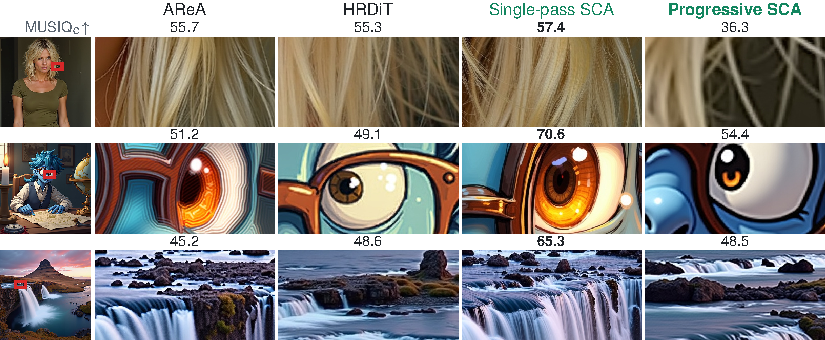
\includegraphics[width=\linewidth]{figures/zoom4k.pdf}
  \caption{\textbf{Single-pass \sca{} keeps the most native detail.} Three Aesthetic-4K evaluation prompts at seed~0: progressive \sca{}'s image with a red window, then that window at 1:1 from each method under its image's MUSIQ$_\text{c}$ (best bold). Progressive \sca{} is softer than single-pass \sca{} in every crop, the fidelity trade-off of Section~\ref{sec:main}.}
  \label{fig:qual_main}
\end{figure}
}

\paragraph{Against HRDiT.} Before correction for multiple comparisons, progressive \sca{} is significantly better on HPSv2, MUSIQ, and ARNIQA, worse only on CLIP-IQA, and within noise on the other six per-image metrics (Table~\ref{tab:prog_deltas}).\IfFileExists{figures/snippets/app_tables/holm.tex}{ After a Holm correction over the ten per-image metrics, \ifdefined\holmProgHrditKept\holmProgHrditKept\else HPSv2 and ARNIQA\fi{} remain and no metric is worse (Table~\ref{tab:holm}).}{} HRDiT has lower KID, patch FID (103.0 against 107.7; progressive minus HRDiT $+4.6$ $[0.6,7.7]$), and patch KID, while the FID difference (141.9 against 138.4) spans zero. Progressive \sca{} takes 49.2\,s per image and HRDiT 107.0\,s in run T3, and 50.7 and 110.4\,s as campaign means on shared nodes.\ifvsnip{crops_matched}{ Where the four methods draw the same content, progressive \sca{}'s crop detail is level with HRDiT's (Figure~\ref{fig:crops_matched}); over all \nmain{} prompts the MUSIQ over four $1024^2$ crops differ by $\hlProgHrditMusiqc$ $[\hlProgHrditMusiqcLo,\hlProgHrditMusiqcHi]$.}{}

\paragraph{Against single-pass \sca{}.} Progressive \sca{} gains seven per-image metrics, ties on CLIP ($+0.25$ $[-0.02,0.52]$), and loses both MUSIQ scores (Table~\ref{tab:prog_deltas}).\IfFileExists{figures/snippets/app_tables/holm.tex}{ Its ImageReward gain is the weakest of the seven: it survives the Holm correction with bootstrap $p$-values but not with the sign-flip test (Table~\ref{tab:holm}).}{} Its patch FID ($+9.2$ $[5.1,13.2]$) and patch KID are significantly higher, and its FID and KID differences span zero. It takes 27.7\,s less per image in campaign means (50.7 against 78.4\,s) and 27.9\,s less in clean times (49.2 against 77.1\,s). Figure~\ref{fig:progressive} shows that progressive \sca{} keeps a large subject, as HRDiT does, while single-pass \sca{} draws it smaller. Figure~\ref{fig:qual_main} compares five methods crop by crop, and Figure~\ref{fig:gallery_prog} sets the two modes side by side on six more prompts.


% =====================================================================================
\apxbarrier
\section{Generality}
\label{app:generality}

This appendix expands Table~\ref{tab:generality} and Section~\ref{sec:generality}. Table~\ref{tab:gen_all} expands every row of Table~\ref{tab:generality} to all ten per-image metrics with intervals (Appendix~\ref{app:gen_seeds}). Appendix~\ref{app:gen_krea} covers $6144^2$ and FLUX.1-Krea-dev, Appendix~\ref{app:wide} the non-square sizes, and Appendix~\ref{app:8k} the exploratory $8192^2$ run\ifanynewmodel; Appendix~\ref{app:newer} adds the newer models\fi.

\subsection{Seeds, HRGen-1K, and FLUX.2-dev}
\label{app:gen_seeds}

Table~\ref{tab:gen_all} gives every row of Table~\ref{tab:generality} on all ten per-image metrics with intervals: progressive \sca{} against AReA at three seeds and on HRGen-1K; single-pass \sca{} against AReA on HRGen-1K, at seeds 1 and 2, and on FLUX.1-Krea-dev; and \sca{} without the schedule against full attention on FLUX.2-dev (Appendix~\ref{app:additional_protocols}). Table~\ref{tab:prog_all} expands the progressive row at seed 0 to every metric. Figure~\ref{fig:gallery_flux2} shows four FLUX.2-dev prompts; FLUX.2-dev runs at guidance 4.0 with its own reach table.

% tab:phase2_general (v5.1) is retired: Table G.1 holds every one of its numbers. The label stays as an alias.
\apxalias{tab:gen_all}{tab:phase2_general}
\snippetat{!htbp}{app_tables/gen_all}

\apxcap{1}{FLUX.2-dev at $4096^2$: \sca{} without the schedule against full attention; in the portrait \sca{} distorts facial geometry and fine texture.}{Over the 50 FLUX.2-dev prompts, \sca{} without the schedule is significantly better than full attention on \hlFluxTwoWinsWord{} of ten per-image metrics, both MUSIQ scores among them (Table~\ref{tab:gen_all}).}
\vsnippetcap{!htbp}{gallery_flux2}

\subsection{\texorpdfstring{$6144^2$}{6144x6144} and FLUX.1-Krea-dev}
\label{app:gen_krea}

Table~\ref{tab:krea_6144} gives every metric with its paired interval for the 100-prompt $6144^2$ comparison, which uses \sca{} without the schedule, and for FLUX.1-Krea-dev. On FLUX.1-Krea-dev, DyPE and SEGA trail AReA on ImageReward, and single-pass \sca{} does not. The Krea reach table follows the FLUX.1-dev procedure with 16 prompts at $1024^2$ (Appendix~\ref{app:area}). The progressive sampler does not support FLUX.1-Krea-dev, so every Krea row is single-pass \sca{}.

Figure~\ref{fig:gallery_6144_complete} shows four $6144^2$ prompts, and Figure~\ref{fig:gallery_krea_complete} two FLUX.1-Krea-dev prompts with AReA, DyPE, SEGA, and single-pass \sca{}. The Krea images use the FLUX.1-Krea-dev transformer with FLUX.1-dev text encoders and VAE and a reach table fitted on FLUX.1-Krea-dev. Their DyPE and SEGA images come from the recorded FLUX.1-Krea-dev evaluation runs. In those runs seven SEGA outputs were regenerated from an archived runtime because their original source snapshots could not be recovered\ifvsnip{gallery_krea_complete}{; neither prompt shown is among them}{}. The inherited Krea baselines span several runtime revisions.

\snippetat{!htbp}{app_tables/krea_6144}
\apxcap{1}{At $6144^2$ both methods show artifacts: dots for AReA, blocks for \sca{} without the schedule.}{Over the 100 prompts, \sca{} without the schedule is better than AReA on \hlSixKWins{} of 15 metrics (Table~\ref{tab:krea_6144}).}
\vsnippetcap{!htbp}{gallery_6144_complete}
\apxcap{1}{AReA, DyPE, SEGA, and single-pass \sca{} on FLUX.1-Krea-dev.}{Over all \nkrea{} prompts, single-pass \sca{} is significantly better than AReA on \hlKreaWinsWord{} of ten per-image metrics and worse on none; its ImageReward difference, $\hlKreaIr$ $[\hlKreaIrLo,\hlKreaIrHi]$, includes zero (Table~\ref{tab:krea_6144}).}
\vsnippetcap{!htbp}{gallery_krea_complete}

\subsection{Non-square sizes}
\label{app:wide}

Table~\ref{tab:app_wide} pairs single-pass \sca{} with AReA at $2048\times4096$ and $2048\times6144$. At $2048\times4096$ the window already covers half the image height, so the per-head mix gains little (Appendix~\ref{app:failures}); Appendix~\ref{app:ps2} checks which reach table that size should read.

\begin{table}[!htbp]
  \caption{\textbf{At $2048\times6144$ single-pass \sca{} wins seven of 15 metrics; at $2048\times4096$ the result is mixed.} Expands the aspect-ratio paragraph of Section~\ref{sec:sizes}. FLUX.1-dev, \nmain{} prompts each; AReA runs its released code. $\Delta$: single-pass \sca{} minus AReA, with its 95\% paired percentile-bootstrap interval in grey over 1000 prompt draws; for FID, KID, and their patch versions the draws also resample reference-image clusters. \up{Blue} / \dn{orange}: significantly better / worse than AReA; for FID, KID, and time lower is better. $^\ddagger$Campaign mean on shared nodes. Key result: at $2048\times6144$ single-pass \sca{} wins seven of 15 metrics and loses two, at $2048\times4096$ it wins three and loses three, and it is faster at both.\pendAppWide}
  \label{tab:app_wide}
  \apxbody{app_tables/app_wide}
\end{table}

\subsection{Exploratory \texorpdfstring{$8192^2$}{8192x8192} comparison}
\label{app:8k}

This subsection expands the $8192^2$ sentence of Section~\ref{sec:sizes}. Table~\ref{tab:e2_8192_per_image} reports all 12 completed prompt pairs at $8192^2$ under the shared FLUX.1-dev protocol, for \sca{} without the schedule against AReA. \sca{} without the schedule has higher ImageReward, CLIP, PickScore, both HPS variants, and ARNIQA, with paired intervals that exclude zero. Aesthetic score and the three remaining quality metrics have intervals that span zero, and MUSIQ, MUSIQ$_\text{c}$, and CLIP-IQA have point estimates that favour AReA. These mixed quality scores and the grid and stripe failures in Figure~\ref{fig:gallery_8192_complete} limit the evidence for reliable 8K generation. With only 12 prompts the comparison is exploratory, and we report no distribution metrics for it.

\snippetat{!htbp}{e2_8192_tables}
\apxcap{1}{At $8192^2$ both methods show artifacts: dots and grids for AReA, stripes and blocks for \sca{} without the schedule.}{Over the 12 prompts, \sca{} without the schedule is significantly better than AReA on \hlEightKFavWord{} of ten metrics (Table~\ref{tab:e2_8192_per_image}).}
\vsnippetcap{!htbp}{gallery_8192_complete}

All 8K scores were computed on CPU (Table~\ref{tab:e2_8192_per_image} notes the HPS precision). For native-resolution MUSIQ, attention queries are processed in chunks of 256 while every key and native image patch is retained. This bounds intermediate memory without changing the attention context; equivalence checks with the pretrained model at three smaller image sizes reproduced the unchunked scores exactly.


% Newer models: each block appears only when its switch is on in main.tex (snippets written by the run owners).
\ifanynewmodel
\subsection{Newer models}
\label{app:newer}

This subsection expands the newer-model paragraphs of Section~\ref{sec:generality}.\ifresfluxtwo{} Figure~\ref{fig:showcase_flux2} shows \sca{} on FLUX.2-dev.\fi\ifresqwen{} Figure~\ref{fig:showcase_qwen} shows \sca{} on Qwen-Image.\fi\ifresideogram{} \ideogramRefs{} cover Ideogram~4 at $8192^2$.\fi

\ifresfluxtwo\snippet{showcase_flux2}{}\fi
\ifresqwen\snippet{showcase_qwen}{}\fi
\ifresideogram\snippet{ideogram4}{}\snippet{ideogram4_fig}{}\fi
\fi

% =====================================================================================
\apxbarrier
\section{Sensitivity and budgets}
\label{app:budget}

This appendix tests the settings that the main text fixes, and expands the sensitivity sentence of Section~\ref{sec:generality} and the SigMa comparison of Section~\ref{sec:main}. Appendix~\ref{app:sens} varies the number of emulation prompts and the gate, Appendix~\ref{app:ps2} the table read at a non-square size, and Appendix~\ref{app:budgets} the number of steps and the guidance.

\subsection{Emulation budget and gate}
\label{app:sens}

We merge the stored sufficient statistics of the first 4, 8, or 16 emulation prompts and rerun the \nabl{} ablation prompts with each resulting table. Table~\ref{tab:phase2_sensitivity} reports the generation-level differences from the 32-prompt table, all for \sca{} without the schedule, together with two other gates. The test reuses the emulation statistics but evaluates on separate prompts; it is not a held-out output-error benchmark. Tables fitted on 4 to 16 prompts change one of 30 differences significantly. A gate at $\sigma_g=0.85$ lowers seven metrics, and a gate at $0.93$ lowers CLIP score and PickScore and raises ARNIQA.

\apxfloat{app_tables/phase2_sensitivity}{tab:phase2_sensitivity}

\subsection{Reach table at non-square sizes}
\label{app:ps2}

This subsection checks the ratio rule of Section~\ref{sec:emulation} at a non-square size. At $(s_H,s_W)=(2,4)$ the two axes have different factors, and the native phase reads the table of the ratio nearest the larger factor, ratio 4. On the \nabl{} ablation prompts at $2048\times4096$, for \sca{} without the schedule, the ratio-2 table makes three significant changes, all at most 0.17 (Table~\ref{tab:app_ps2}): HPSv2 $+0.09$, HPSv2.1 $+0.17$ (both $\times100$), and PickScore $+0.05$. ImageReward ($+0.01$ $[-0.03,0.05]$) and the other metrics are within noise. Changes this small cannot resolve the mixed results of single-pass \sca{} against AReA at this size, so we keep the default rule.

\apxfloat{app_tables/app_ps2}{tab:app_ps2}

\subsection{Sampling budgets, guidance, and SigMa}
\label{app:budgets}

Table~\ref{tab:panel46} adds SigMa and three budgets of \sca{} without the schedule to Table~\ref{tab:main}. Table~\ref{tab:phase2_budget} gives the budget and guidance checks with intervals, and Figure~\ref{fig:quality_time} plots ImageReward against time.

\begin{table}[!htbp]
  \caption{\textbf{SigMa trails single-pass \sca{} on every metric shown; 56 steps raise the ImageReward of \sca{} without the schedule by 0.03 at twice the time.} \npanel{} prompts at $4096^2$. s: campaign mean in seconds per image on shared nodes, which every row has; IR ImageReward, HPSv2.1 $\times100$, Pick PickScore, M$_\text{c}$ MUSIQ on four $1024^2$ crops, FID$_\text{p}^\dagger$ our patch FID (Appendix~\ref{app:metricdefs}). Bold: best, underline: second within each group; shaded: ours. Colours mark each row against single-pass \sca{} at 28 steps; the budget rows use \sca{} without the schedule and are coloured against its 28-step run, which this table does not show (Table~\ref{tab:phase2_budget}). The FID cells of SigMa and single-pass \sca{} have no interval. Table~\ref{tab:main} holds the multi-stage rows. Key result: 56 steps take 139.9 against 71.5\,s per image.}
  \label{tab:panel46}
  \centering\footnotesize
  \apxbody{main_tables/tab_panel46}
\end{table}

% Table H.4 is defined before the wrapped paragraphs so that no float lands inside the wrap.
\apxfloat{app_tables/phase2_budget}{tab:phase2_budget}

% The quality-time plot at half width with its caption beside it (a normal float; a wrapfigure collided with the
% neighbouring tables).
\begin{figure}[!htbp]
  \centering
  \begin{minipage}[c]{0.5\linewidth}
    \IfFileExists{figures/v6/quality_time.pdf}{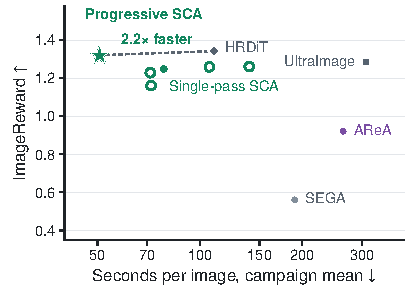
\includegraphics[width=\linewidth]{figures/v6/quality_time.pdf}}{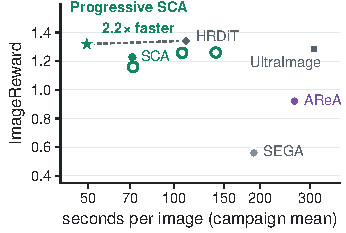
\includegraphics[width=\linewidth]{figures/quality_time_wrap.pdf}}
  \end{minipage}\hfill
  \begin{minipage}[c]{0.46\linewidth}
    \captionsetup{justification=raggedright,singlelinecheck=false}
    \caption{\textbf{At \hlCampProgHrditPct\% of HRDiT's time, progressive \sca{} is indistinguishable from HRDiT on ImageReward (difference $\hlProgHrditIr$ $[\hlProgHrditIrLo,\hlProgHrditIrHi]$).} ImageReward against campaign seconds per image on shared nodes, $n=\npanel$ prompts at $4096^2$. Star: progressive \sca{}; filled circle: single-pass \sca{}; open circles: \sca{} without the schedule at 28, 42, and 56 steps and at guidance 7; the dashed guide carries the ratio of campaign times. Full attention, DyPE, and SigMa fall below the range (Table~\ref{tab:panel46}).}
    \label{fig:quality_time}
  \end{minipage}
\end{figure}

\paragraph{SigMa.} With its dev-matched profile (Appendix~\ref{app:additional_protocols}), SigMa trails single-pass \sca{} on all ten per-image metrics (Table~\ref{tab:panel46_deltas}) and takes 192.5\,s per image against 78.4\,s (campaign means).

\paragraph{More steps and higher guidance.} On the same \npanel{} prompts we compare the default 28-step run of \sca{} without the schedule with 56 steps at guidance 4.5 and with 28 steps at guidance 7 (Table~\ref{tab:phase2_budget}). The 56-step run keeps the noise threshold at 0.89, so it changes the discretization of both the opening and the mixed phase. It improves ImageReward by 0.032 $[0.0002,0.062]$, HPSv2.1 by 0.88, PickScore by 0.13, and MUSIQ$_\text{c}$ by 2.9. It also raises corrected patch FID by 3.85 $[1.51,6.33]$ under reference-cluster resampling. Guidance 7 alone lowers seven per-image metrics, ImageReward by 0.068 $[0.025,0.115]$ among them, and raises only MUSIQ. The default settings therefore do not maximize every metric: 56 steps gain eight per-image metrics but raise patch FID by 3.85.

\paragraph{Against UltraImage and HRDiT.} On these \npanel{} prompts, 56-step \sca{} without the schedule differs from UltraImage by $-0.023$ $[-0.089,0.040]$ in ImageReward, $-0.22$ $[-0.51,0.05]$ in HPSv2.1, and $-0.11$ $[-0.21,-0.01]$ in PickScore. The first two intervals span zero and do not establish equivalence; PickScore favours UltraImage. The MUSIQ advantage of 56-step \sca{} without the schedule is 11.6 $[9.5,13.6]$, and its MUSIQ$_\text{c}$ advantage 22.4 $[21.2,23.6]$. Campaign means are 71.5\,s for 28 steps, 139.9\,s for 56 steps, and 308.5\,s for UltraImage. This check matches neither FLOPs nor wall-clock time: UltraImage takes 308.5 against 139.9\,s, runs two resolutions with different guidance, and needs per-prompt preparation. Against HRDiT on the same prompts (Table~\ref{tab:main}), the 56-step run stays lower on ImageReward (1.26 against 1.34), HPSv2.1 (30.55 against 30.92), and PickScore (23.22 against 23.46). It also takes longer (139.9 against 110.4\,s). These are point estimates without paired intervals.

\paragraph{A 42-step run.} Table~\ref{tab:prog_deltas} adds a 42-step run of \sca{} without the schedule, sized to HRDiT's campaign time (106.8 against 110.4\,s). The extra steps raise PickScore, HPSv2, HPSv2.1, ARNIQA, and MUSIQ$_\text{c}$ over 28 steps but leave ImageReward unresolved. HRDiT stays significantly ahead of the 42-step run on ImageReward, PickScore, HPSv2.1, aesthetic score, and CLIP-IQA, and trails it on both MUSIQ scores and ARNIQA. With \npanel{} generated images, 168 reference identities, and 1000 bootstrap draws, the 42-step run has significantly higher FID than the 28-step run ($+2.4$ $[0.1,5.7]$); KID, patch FID ($+1.5$ $[-0.5,3.6]$), and patch KID span zero. Appendix~\ref{app:prog} runs \sca{} inside HRDiT's schedule instead.


% =====================================================================================
\apxbarrier
\section{Compute and reproducibility}
\label{app:compute}

This appendix expands the reproducibility statement. Appendix~\ref{app:hardware} gives the hardware and the logged compute, and Appendix~\ref{app:release} lists what the code release contains and where each reported number comes from.

\subsection{Hardware and compute}
\label{app:hardware}

Generation and reach emulation used single NVIDIA GH200 GPUs on a shared cluster; the verified timing logs identify the GH200 120\,GB model. Some metric evaluations ran on CPUs. The surviving logs do not establish the complete emulation runtime. At $4096^2$ on shared nodes, campaign means are about 51\,s per image for progressive \sca{} and 78\,s for single-pass \sca{} (Table~\ref{tab:main}). They are 72\,s for \sca{} without the schedule (Appendix~\ref{app:budgets}), 264\,s for AReA, and 196\,s for full attention. The main comparisons, ablations, and non-square sizes comprise more than 2000 generated images. Surviving worker logs establish a lower bound of 123.3 GH200 worker-hours up to 2026-10-17 06:59 UTC, including model loading, reach emulation, evaluation, and failed attempts. Later runs, among them single-pass and progressive \sca{} on all prompts, are not in this bound. The bound is the union of 581 closed task intervals per physical node, with timestamp precision treated conservatively. It measures occupied worker time, not GPU kernel activity. Missing logs, unmatched starts, and ongoing work prevent a complete total, and overlapping scheduler allocation time and per-image durations are not added to the bound.

\subsection{Release and sources}
\label{app:release}

We will release the code: the attention processor, reach emulation, single-pass and progressive sampling, evaluation wrappers, the AReA wrapper, and tests. We will also release the FLUX.1-dev reach table, the per-image metric files, and the per-comparison summary and paired-difference files behind every table. The metric values and paired intervals of the paper are derived from those files. Each \sca{} generation task ran from a frozen copy of the code named in the task. Per-image records store the sampling settings and, where available, a code fingerprint; the inherited FLUX.1-Krea-dev baseline records do not establish one source revision for every image. Table~\ref{tab:sources} maps each item to its file.

\begin{table}[!htbp]
  \caption{\textbf{Every configuration, check, and timing of this appendix maps to a released file.} Paths are relative to the repository root; \texttt{*} stands for a family of files.}
  \label{tab:sources}
  \centering\footnotesize
  \setlength{\tabcolsep}{4pt}
  \begin{tabular}{@{}>{\raggedright\arraybackslash}p{0.33\linewidth}>{\raggedright\arraybackslash}p{0.63\linewidth}@{}}
    \toprule
    Item & File \\
    \midrule
    Single-pass \sca{} (Table~\ref{tab:hparams}) & \texttt{scripts/\allowbreak sample.py -{}-method sca -{}-gate-sigma 0.89 -{}-bridge-cells 8 -{}-bridge-k 16 -{}-win-sched 0.88:128,\allowbreak 0.86:112,\allowbreak 0.84:96,\allowbreak 0.82:80 -{}-win-pi-match -{}-win-pi-interp -{}-pi-table k1\_1024.npz}, code commit \texttt{7bd64c0} \\
    Progressive \sca{} (Algorithm~\ref{alg:prog}) & \texttt{scripts/\allowbreak sample\_progressive.py} \\
    Reach emulation and \sca{} attention (Algorithms~\ref{alg:emulate_full} and~\ref{alg:sample_full}) & the statistics and attention modules in \texttt{sca/}; one attention call in \texttt{sca/\allowbreak attn.py} \\
    FLUX.1-dev reach table and statistics & \texttt{calib/\allowbreak k1\_1024.npz}, \texttt{calib/\allowbreak k1\_1024.json} \\
    Numerical checks (Appendix~\ref{app:kernel}) & \texttt{tests/\allowbreak test\_sca.py} (18 CPU tests); \texttt{scripts/\allowbreak bench\_attn.py} (GPU, bf16) \\
    UltraImage wrapper & \texttt{scripts/\allowbreak run\_ultraimage.py} \\
    DyPE and SEGA runner & frozen at commit \texttt{c05ebdc}, recorded in \texttt{repro/\allowbreak README.md} \\
    Corrected crop assembly (Appendix~\ref{app:metricdefs}) & \texttt{repro/\allowbreak evaluate\_corrected.py} \\
    \midrule
    Timing, run T1 & \texttt{results/\allowbreak latency\_curve\_batch1.csv} (with the excluded warm-up images); \texttt{results/\allowbreak latency\_curve\_summary.csv} (every cell but full attention at $6144^2$) \\
    Timing, run T2 & \texttt{results/\allowbreak latency\_curve\_v2/\allowbreak summary.csv} \\
    Timing, run T3 & \texttt{results/\allowbreak prog\_latency/\allowbreak latency\_summary.csv} \\
    Separate $4096^2$ run & \texttt{results/\allowbreak latency\_4096\_batch1.csv} \\
    Table~\ref{tab:app_abl} & \texttt{results/\allowbreak ablnb\_*} and \texttt{calib/\allowbreak k1\_1024.json} \\
    Table~\ref{tab:app_ps2} & \texttt{results/\allowbreak ps2\_*} \\
    Set-level intervals of progressive \sca{} & \texttt{results/\allowbreak prog195\_vs\_baselines/\allowbreak cfid} \\
    Distribution metrics of the 42-step run & \texttt{results/\allowbreak a4k195\_panel/\allowbreak corrected\_fidp\_ci/\allowbreak paired\_deltas.csv} \\
    Sample figures & \ifvsnip{all_methods}{\texttt{paper/\allowbreak figures/\allowbreak v6/\allowbreak *\_provenance.json} beside each figure: selection rule and seed, sources, crop windows}{\texttt{provenance.json} beside each gallery: selection seed, source hashes, crop coordinates} \\
    \bottomrule
  \end{tabular}
\end{table}

% =====================================================================================
\apxbarrier
\section{Limitations in detail}
\label{app:limits}

This appendix expands the limitations of Section~\ref{sec:limits}. Appendix~\ref{app:failures} shows local failures and states the scope of each result, and Appendix~\ref{app:impact} gives the broader impact.

\subsection{Failure cases and scope}
\label{app:failures}

\ifvsnip{failures}{Figure~\ref{fig:failures} shows the four prompts, among those that name no person, on which \sca{} without the schedule trails AReA most in ImageReward, each with AReA's image of the same prompt.}{Figure~\ref{fig:failures} shows four local errors of \sca{} without the schedule next to AReA's same windows.}

\vsnippet{!htbp}{failures}

\paragraph{Hand-set settings.} Only the mixing weight is fitted. The gate, the window sizes, the tile, the bridge, the emulated ratios, and the noise bins are set by hand (Table~\ref{tab:handset}), because output error cannot see layout (Appendix~\ref{app:emu_error}). The window sizes were set on the 46-prompt subset, which is part of the evaluation set (Appendix~\ref{app:protocol}).

\paragraph{Patch fidelity.} Progressive \sca{}'s patch FID is higher than HRDiT's ($+4.6$ $[0.6,7.7]$) and single-pass \sca{}'s ($+9.2$ $[5.1,13.2]$), and higher than AReA's at seeds 0 and 2 (Tables~\ref{tab:prog_all} and~\ref{tab:prog_deltas}).\ifresprogabl{} Inside the progressive sampler the per-head weights win every per-image metric by small margins, while the shared and per-layer weights have lower patch FID (Table~\ref{tab:prog_abl_all}).\fi

\paragraph{Dependence on HRDiT's sampler.} Progressive \sca{} uses HRDiT's sampler, which does not support FLUX.1-Krea-dev. The $6144^2$, $8192^2$, FLUX.2-dev, and sensitivity results use \sca{} without the schedule.

\paragraph{Small factors.} At $2048\times4096$ the window covers half the image height, so the local branch alone already sees most of the image along that axis. There the per-head mix gains little over AReA's shrinking windows, and single-pass \sca{} is significantly worse on aesthetic score, CLIP score, and CLIP-IQA (Table~\ref{tab:app_wide}).

\paragraph{Larger scales and another backbone.} Both use \sca{} without the schedule. The samples of the completed 12-prompt $8192^2$ run still show failures in both methods, speckle for AReA and blocks and stripes for \sca{} without the schedule (Figure~\ref{fig:gallery_8192_complete}); this exploratory set does not establish general 8K quality. In FLUX.2-dev, improved aggregate metrics coexist with distortions of facial geometry and fine texture in the portrait example of Figure~\ref{fig:gallery_flux2}.

\paragraph{Emulation.} Reach emulation omits the bridge and sees 16 times fewer keys per view than the target, so the deployed operator's error is untested.

\paragraph{Text-image offsets.} The local branch keeps out-of-range text-image offsets (Remark~\ref{rem:text}).

\paragraph{Metrics.} No-reference quality metrics reward sharpness even where the layout fails. The variant without the opening phase, which mixes both views with the per-head weights from the first step, scores higher on CLIP-IQA and ARNIQA (Table~\ref{tab:app_abl}). FID against 195 references at $299^2$ resolution sees little of the 4K detail. We therefore report every metric and the qualitative galleries.

\subsection{Broader impact}
\label{app:impact}

\sca{} shortens generation at $4096^2$ relative to full attention under our measured protocol, which helps applications such as print, design, and scientific visualization. Energy use remains unmeasured. The same reduction lowers the cost of producing high-resolution synthetic images that could be used to mislead. \sca{} adds no capability beyond the base model's and does not change its safety filters or watermarking; the risks and mitigations of the base model apply unchanged.

% =====================================================================================
\apxbarrier
\section{Emulation prompts}
\label{app:prompts}

This appendix lists the 48 prompts written for reach emulation (Section~\ref{sec:observation} and Algorithm~\ref{alg:emulate}); none is an evaluation prompt (Appendix~\ref{app:protocol}). The $1024^2$ table uses prompts 1 to 32, and the $1280^2$, FLUX.1-Krea-dev, and FLUX.2-dev tables use prompts 1 to 16. Prompts 33 to 48 are spares that no reported table uses.

% 8 pt on 8.8 pt leading keeps the list on one page, so the sample pages start below their intro.
{\fontsize{8}{8.8}\selectfont
\begin{multicols}{2}
\begin{enumerate}[leftmargin=2.1em,itemsep=0pt,topsep=0pt,parsep=0pt]
  \item A candid street portrait of an elderly fisherman with a weathered face and a knitted wool cap, harbor in the background, overcast light
  \item Two children laughing while running through a lawn sprinkler on a summer afternoon, backlit by the sun
  \item A professional headshot of a young woman with curly red hair and freckles, soft studio lighting, neutral grey backdrop
  \item A jazz trio performing in a dim basement club, saxophone player in the foreground, warm stage lights and haze
  \item A chef plating a dessert in a busy restaurant kitchen, steam rising, stainless steel counters
  \item A ballet dancer mid-leap in an empty rehearsal studio with tall windows and wooden floors
  \item A red fox standing in fresh snow at the edge of a birch forest, early morning light
  \item A macro photograph of a honeybee covered in pollen on a purple lavender flower
  \item A herd of elephants crossing a dusty savanna river at sunset, long shadows
  \item A tabby cat sleeping curled up on a stack of old books next to a window
  \item A school of tropical fish swimming around a coral reef, sun rays through clear blue water
  \item A bald eagle perched on a dead pine branch above a misty lake
  \item A neon sign reading ``OPEN 24 HOURS'' in the window of a rainy diner at night, reflections on the wet sidewalk
  \item A hand-painted wooden sign that says ``Fresh Eggs'' leaning against a farm fence, chickens nearby
  \item A vintage movie theater marquee with the words ``NOW SHOWING'' lit by hundreds of bulbs
  \item A chalkboard menu in a cafe listing coffee drinks and prices in neat handwriting
  \item A highway road sign reading ``Exit 42 Pine Valley'' against a clear blue sky
  \item A bookstore storefront with gold lettering ``Second Chapter Books'' on the glass, autumn leaves on the ground
  \item A wide alpine valley with a winding river, snow-capped peaks and wildflower meadows, midsummer
  \item Sand dunes in the desert at golden hour with sharp ridges and wind ripples
  \item A rugged coastline with sea stacks and crashing waves under a stormy sky
  \item A terraced rice field on a hillside in morning fog, farmers in conical hats
  \item The northern lights over a frozen lake with a small wooden cabin, stars visible
  \item A dense tropical rainforest with a waterfall and hanging vines, light filtering through the canopy
  \item A cozy Scandinavian living room with a fireplace, sheepskin rug, and large windows showing snow outside
  \item A modern open-plan kitchen with a marble island, pendant lights, and potted herbs
  \item A cluttered artist studio with canvases, paint tubes, brushes in jars, and afternoon sunlight
  \item A grand library reading room with long oak tables, green lamps, and arched ceilings
  \item A small Japanese tatami room with a low table, sliding paper doors, and a garden view
  \item A product photograph of a matte black wristwatch on a slate surface, dramatic side light
  \item A pair of white running shoes floating against a pastel gradient background, studio product shot
  \item A glass bottle of olive oil with a sprig of rosemary on a rustic wooden table, soft daylight
  \item A flat lay of a leather notebook, fountain pen, glasses, and a cup of espresso on a desk
  \item A ceramic teapot with a blue glaze and matching cups arranged on a linen tablecloth
  \item A crowded night market in Taipei with food stalls, lanterns, and hundreds of people
  \item A packed football stadium during a night match, floodlights and cheering fans
  \item Commuters crossing a huge intersection in Tokyo during rush hour, seen from above
  \item A music festival crowd at sunset with raised hands and confetti in the air
  \item A busy train station concourse with travelers, departure boards, and a glass roof
  \item A gothic cathedral facade with intricate stone carvings and a rose window, low angle
  \item A row of colorful Victorian townhouses on a hilly street with a cable car
  \item A brutalist concrete apartment block with repeating balconies under a pale sky
  \item A glass skyscraper reflecting clouds, shot looking straight up from the street
  \item A traditional Chinese pagoda beside a lake with cherry blossoms in full bloom
  \item An old stone bridge over a canal in Venice with gondolas and laundry lines
  \item An astronaut riding a horse across a red desert planet with two moons, cinematic
  \item A detailed watercolor illustration of a lighthouse on a rocky island with seagulls
  \item A steampunk airship floating above a Victorian city at dusk, intricate brass details
\end{enumerate}
\end{multicols}}

% =====================================================================================
\section{Sample pages}
\label{app:galleries}

\ifvsnip{all_methods}{%
This appendix expands Figures~\ref{fig:prog_hero} and~\ref{fig:qual_prog} with full pages of samples; Appendix~\ref{app:samples} gives the selection and crop rules. Figure~\ref{fig:gallery_prog} sets both modes of \sca{} beside AReA, UltraImage, and HRDiT on six prompts, and Figure~\ref{fig:teaser} shows eight methods on two more. Figures~\ref{fig:gallery_prog16} and~\ref{fig:gallery_prog16b} set progressive \sca{} beside AReA, UltraImage, and HRDiT on 18 prompts. Figure~\ref{fig:hero} shows single-pass \sca{} at three aspect ratios, and Figures~\ref{fig:gallery_4096} to~\ref{fig:gallery_6144x2048} set it beside AReA on 16 prompts at $4096^2$ and four at each wide size.}{%
This appendix expands Figures~\ref{fig:prog_hero} and~\ref{fig:qual_prog} with full pages of samples; Appendix~\ref{app:samples} gives the selection and crop rules. Figure~\ref{fig:gallery_prog} shows six prompts with every method, and Figure~\ref{fig:teaser} six methods on one prompt. Figures~\ref{fig:gallery_prog16} and~\ref{fig:gallery_prog16b} set progressive \sca{} beside AReA and HRDiT on sixteen prompts. Figure~\ref{fig:hero} shows single-pass \sca{} at three aspect ratios, and Figures~\ref{fig:gallery_4096} to~\ref{fig:gallery_6144x2048} set it beside AReA at $4096^2$, $2048\times4096$, and $2048\times6144$.}\ifshowcase{} Figure~\ref{fig:showcase_models} shows \sca{} on FLUX.2-dev and Qwen-Image.\fi

% Sample pages: the first sits below the intro when it fits, the others fill pages of their own, top-aligned
% (\topfloatpages). The smaller sample figures sit beside their tables in Appendices E and G.
\apxcap{1}{Both modes of \sca{} beside AReA, UltraImage, and HRDiT at $4096^2$.}{Over all \nmain{} prompts, progressive minus single-pass \sca{} is $\hlProgScaMusiqc$ $[\hlProgScaMusiqcLo,\hlProgScaMusiqcHi]$ on MUSIQ over four $1024^2$ crops and $\hlProgScaIr$ $[\hlProgScaIrLo,\hlProgScaIrHi]$ on ImageReward (Table~\ref{tab:prog_deltas}).}
\vsnippetcap{!ht}{gallery_prog}
\apxcap{1}{Full attention loses the scene and DyPE and SEGA overlay a lattice; the other five keep it.}{Over all \nmain{} prompts, full attention, DyPE, and SEGA each trail progressive \sca{} on all ten per-image metrics (Table~\ref{tab:prog_all}).}
\ifvsnip{all_methods}{\vsnippetcap{p}{all_methods}}{%
\begin{figure}[!htbp]
  \centering
  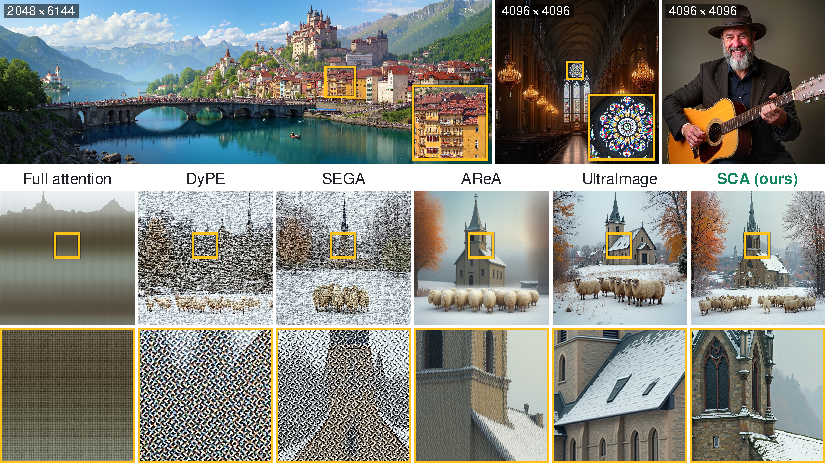
\includegraphics[width=\linewidth,trim=0 0 0 1.12in,clip]{figures/teaser.pdf}
  \caption{\textbf{Six methods on one $4096^2$ prompt.} Single-pass \sca{}; each column shows the image and a 1:1 crop. Full attention gives a flat field, DyPE and SEGA a lattice, and the other three keep the church and the flock. Aesthetic-4K evaluation prompt at seed~0; Figure~\ref{fig:gallery_4096} shows more prompts.}
  \label{fig:teaser}
\end{figure}
}
\apxcap{1}{Progressive \sca{} beside AReA, UltraImage, and HRDiT at $4096^2$, prompts 1 to 9 of 18.}{Over all \nmain{} prompts, progressive \sca{}'s MUSIQ over four $1024^2$ crops exceeds AReA's by $\hlProgAreaMusiqc$ $[\hlProgAreaMusiqcLo,\hlProgAreaMusiqcHi]$ and UltraImage's by $\hlProgUltraMusiqc$ $[\hlProgUltraMusiqcLo,\hlProgUltraMusiqcHi]$, and is indistinguishable from HRDiT's ($\hlProgHrditMusiqc$ $[\hlProgHrditMusiqcLo,\hlProgHrditMusiqcHi]$; Table~\ref{tab:prog_all}).}
\apxcap{2}{Progressive \sca{} beside AReA, UltraImage, and HRDiT at $4096^2$, prompts 10 to 18 of 18.}{}
\vsnippetcap{p}{gallery_prog16}
\apxcap{1}{Single-pass \sca{} at three aspect ratios with one reach table.}{Against AReA, single-pass \sca{} wins \hlWideSixWins{} metrics at $2048\times6144$, and wins \hlWideFourWinsWord{} and loses \hlWideFourLossesWord{} at $2048\times4096$ (Table~\ref{tab:app_wide}).}
\vsnippetcap{p}{hero}
\ifshowcase\apxcap{1}{The same six prompts on three models.}{}\vsnippetcap{p}{showcase_models}\fi
\apxcap{1}{Single-pass \sca{} beside AReA at $4096^2$, prompts 1 to 8 of 16.}{Over all \nmain{} prompts, single-pass \sca{} is significantly better than AReA on all ten per-image metrics\ifdefined\hlScaAreaMusiqc, MUSIQ over four $1024^2$ crops by $\hlScaAreaMusiqc$ $[\hlScaAreaMusiqcLo,\hlScaAreaMusiqcHi]$\else, both MUSIQ scores among them\fi{} (Table~\ref{tab:app_4k}).}
\vsnippetcap{p}{gallery_4096}
\apxcap{1}{Single-pass \sca{} beside AReA at $4096^2$, prompts 9 to 16 of 16.}{}
\vsnippetcap{p}{gallery_4096_p2}
\apxcap{1}{At $2048\times4096$ both methods keep the layout.}{At this size single-pass \sca{} wins \hlWideFourWinsWord{} of 15 metrics against AReA and loses \hlWideFourLossesWord{} (Table~\ref{tab:app_wide}).}
\vsnippetcap{p}{gallery_4096x2048}
\apxcap{1}{Single-pass \sca{} beside AReA at $2048\times6144$.}{At this size single-pass \sca{} wins \hlWideSixWins{} metrics against AReA, both MUSIQ scores among them (Table~\ref{tab:app_wide}).}
\vsnippetcap{p}{gallery_6144x2048}
